% !TEX root = ../McCoy-Dissertation.tex
\Appendix{On X-ray Reflection}\label{app:x-ray_materials} 
%%%%%%%%%%%%%%%%%%%%%%%%%%%%%%%%%%%%%%%%%--------------------------------------------------
Motivated in \cref{ch:introduction}, x-ray reflection gratings are a technology suitable for sensitive absorption spectroscopy provided that they perform with high diffraction efficiency and high spectral resolving power. 
Although \cref{sec:grating_fab_intro} outlines methods for the manufacture of surface reliefs for x-ray reflection gratings, what is not addressed therein is that achieving an efficient, blazed response from a grating requires a reflective overcoat that takes into account the physics of how soft x-rays interact with matter. 
The principles behind these physical phenomena give insight into which materials and film thicknesses are appropriate for these overcoats under \emph{total external reflection} and additionally, considerations for surface roughness on the grating groove facets. 
Ultimately, reviewing this physics is prudent to understanding how fabricated x-ray reflection gratings can be tested empirically for diffraction efficiency [\emph{cf.\@} \cref{sec:als_testing}] and compared to theoretical models that are based on vector theories of diffraction [\emph{cf.\@} \cref{sec:integral_method}]. 
The goal of this appendix is to provide an overview for the physics of x-ray reflection starting with how soft x-rays propagate through a medium as they interact with atomic electrons in \cref{sec:SXR_med}. 
With an \emph{index of refraction} for soft x-rays formulated from these phenomena, \cref{sec:planar_interface} treats reflection from a mirror flat and discusses how the choice of material for a reflective overcoat and the level of surface roughness produced impacts specular reflectivity; a summary is provided in \cref{sec:appC_summary}. 

\section{Soft X-rays in Materials}\label{sec:SXR_med}
%%%%%%%%%%%%%%%%%%%%%%%%%%%%%%%%%%%%%%%%%--------------------------------------------------
Electromagnetic radiation in vacuum is described classically as coupled oscillations in the electric field $\mathbold{E}(\mathbold{r},t)$ and the magnetic field $\mathbold{B}(\mathbold{r},t)$ that propagate as a wave at the speed of light, $c_0$ [\emph{cf.\@} \cref{sec:EM_waves_vac}]. 
As such an electromagnetic wave propagates inside a material on the other hand, $\mathbold{E}(\mathbold{r},t)$ and $\mathbold{B}(\mathbold{r},t)$ interact with the bound charge density, $\rho_b(\mathbold{r},t)$, and the bound current density, $\mathbfcal{J}_b(\mathbold{r},t)$, associated with the atomic electrons in a manner that varies substantially across the electromagnetic spectrum \cite{Jackson75,Landau60,Griffiths17}. 
Semi-classically, the dominant interactions can be summarized as: 
\begin{enumerate}[noitemsep]
  \item Atomic nuclei and their electrons are forced slightly in opposite directions by $\mathbold{E}(\mathbold{r},t)$, generating an \emph{electric-dipole moment} that is said to be polarized toward the direction of the positive charge. 
  \item The total orbital angular momentum and quantum-mechanical spin of atomic electrons have a small tendency to align with $\mathbold{B}(\mathbold{r},t)$, which induces a net \emph{magnetic-dipole moment} that would otherwise not be there in a non-magnetic material.
\end{enumerate} 
These induced dipole moments are described macroscopically, per unit volume by the \emph{electric polarization field}, $\mathbold{P}(\mathbold{r},t)$, and the \emph{magnetization field}, $\mathbold{M}(\mathbold{r},t)$, which are directly related to $\rho_b(\mathbold{r},t)$ and $\mathbfcal{J}_b(\mathbold{r},t)$ \cite{Jackson75,Landau60,Griffiths17}: 
\begin{subequations}
\begin{equation}\label{eq:electric_polarization_field}
 \rho_b (\mathbold{r},t) \equiv - \div \mathbold{P}(\mathbold{r},t) 
 \end{equation}
\begin{equation}\label{eq:magnetization_field}
 \mathbfcal{J}_b (\mathbold{r},t) \equiv \curl \mathbold{M}(\mathbold{r},t) . 
 \end{equation} 
\end{subequations}
Thus, as $\mathbold{P}(\mathbold{r},t)$ and $\mathbold{M}(\mathbold{r},t)$ are driven by $\mathbold{E}(\mathbold{r},t)$ and $\mathbold{B}(\mathbold{r},t)$ of an electromagnetic wave, $\rho_b(\mathbold{r},t)$ and $\mathbfcal{J}_b(\mathbold{r},t)$ act as source terms in Maxwell's equations [\emph{cf.\@} \cref{eq:Maxwell_vac_start_1,eq:Maxwell_vac_start_2,eq:Maxwell_vac_start_3,eq:Maxwell_vac_start_4}], which describe how more radiation is produced from these interactions. %in a manner similar in concept to a basic radio antenna. 
Then, the overall electromagnetic wave that is \emph{refracted} and \emph{attenuated} as it propagates in the medium with a group velocity smaller than $c_0$ is the superposition of the original wave with these radiated waves, which generally have a phase shift associated with them \cite{Jackson75,Rybicki86,Griffiths17}. 

The above scenario describes the classical, macroscopic effect that scattering from atomic electrons has on wave propagation inside a  material. 
However, it was implicitly assumed that the material could be treated as a continuous medium, or equivalently, that the wavelength of the radiation, $\lambda$, is much larger than the atomic scale, which can be taken as the Bohr radius $a_0 \approx \SI{0.05}{\nm}$ [\emph{cf.\@} \cref{sec:allowed_transitions}]. 
Although this approximation is often valid, for example, in the visible light spectrum, where $\SI{700}{\nm}\gtrapprox \lambda \gtrapprox \SI{400}{\nm}$, it breaks down for soft x-rays and other radiation with $\lambda \lessapprox a_0$  \cite{Landau60,Attwood17,Als-Nielsen11}. 
While this condition comes with its own set of consequences, which are described throughout this appendix, another aspect to consider is the highly frequency-dependent nature of scattering in materials. 
For reference, the frequency, $\omega = 2 \pi c_0 / \lambda$, of visible light is large enough to neglect the magnetic-dipole processes that may come into play for radio waves and other relatively low-frequency radiation but still much smaller than virtually all atomic resonances, which are given by $\omega_e \equiv \mathcal{E}_e / \hbar$, where $\mathcal{E}_e$ is an electronic binding energy \cite{Landau60,Jackson75}. 
That is, with timescales for magnetic-dipole processes being much longer than the timescale $\omega^{-1}$, electric-dipole interactions are the dominant contribution to the scattered radiation from bound electrons with $\omega \ll \omega_e$. 
As frequency increases into the hard x-ray spectrum however, $\omega^{-1}$ is so short that even electric-dipole processes do not have time to respond to the oscillation of the wave and as a result, scattering is characteristic of a free electron with $\omega \gg \omega_e$ \cite{Attwood17,Als-Nielsen11}. 
Importantly, soft x-rays exist in between these two limiting cases, where $\omega$ is in the neighborhood of $\omega_e$ for atomic electrons and hence a more detailed description of scattering should be considered. 

For scattered radiation to interfere constructively and contribute to the overall electromagnetic wave that propagates in a material, the scattering processes must be \emph{coherent} in the sense that $\omega$ for the driving and radiating waves are nominally identical. 
This therefore excludes inelastic processes such as \emph{Compton scattering}, where the incoming photon\footnote{Typically, this is a hard x-ray photon with substantial quantized momentum [\emph{cf.\@} \cref{ap:x-ray_intro}].} transfers momentum to an atomic electron as it ejects it and scatters as a new photon with reduced $\omega$ and increased $\lambda$ \cite{Als-Nielsen11}. 
There then are two main types of coherent scattering alluded to above that are relevant in different scenarios depending on how photon energy, $\mathcal{E}_{\gamma} \equiv \hbar \omega$, compares to $\mathcal{E}_e$ for a given atomic electron: 
\begin{enumerate}[noitemsep]
 \item \emph{Rayleigh scattering} for $\mathcal{E}_{\gamma} \ll \mathcal{E}_e$, where the electron binding force has a strong effect on the interaction (\emph{e.g.}, visible light scattering from virtually any atom). 
 \item \emph{Thomson scattering} for $\mathcal{E}_{\gamma} \gg \mathcal{E}_e$, where the electron binding force is unimportant in the interaction (\emph{e.g.}, hard x-rays scattering from electrons in low-to-mid $\mathcal{Z}$ atoms). 
 \end{enumerate} 
These coherent-scattering processes can be treated quantum-mechanically as the absorption of a photon with $\abs{\mathbold{k}} = k_0 \equiv 2 \pi / \lambda$ coupled with the emission of a new photon with $\abs{\mathbold{k}'} = k_0$ that propagates in a different, probabilistic direction. 

Rayleigh scattering can be described as a second-order perturbation of $\underline{\mathcal{H}}^{(1)} \equiv  \left( q_e / m_e \right) \underline{\mathbold{A}} ( \mathbold{r} ) \cdot \underline{\mathbold{p}}$ [\emph{cf.\@} \cref{sec:ions_EM}], where the relevant time evolution operator for an atomic electron under the \emph{self-consistent field approximation} can be written as\footnote{Here, operators are expressed in the interaction picture using \cref{eq:interaction_operator}.}
\begin{subequations}
\begin{equation}
 \underline{U}_I (t) \approx 1 - \frac{i}{\hbar} \int_0^t \underline{\mathcal{H}}^{(1)}_I (t') \dd{t'} + \left(- \frac{i}{\hbar} \right)^2 \int_0^t \underline{\mathcal{H}}^{(1)}_I (t') \dd{t'} \int_0^{t'} \underline{\mathcal{H}}^{(1)}_I (t'') \dd{t''} ,
 \end{equation}
where the first term describes first-order processes such as bound-bound transitions and \emph{photo-ionization} [\emph{cf.\@} \cref{sec:single_absorption_emission}] while the second-order term can be expanded in terms of a complete set of intermediate electron-photon states ,$\sum_{I} \ket{I} \bra{I}$, where $\ket{I}$ is any possible intermediate electron-photon state. 
Quantum-mechanically, this describes all the possible transitions that the electron can make as it interacts with photons on its way from the initial state $\ket{A}$ to the final state $\ket{B}$ \cite{Townsend00,deBergevin09}. 
The corresponding matrix element (neglecting the first term) then is 
\begin{equation}%\label{eq:second_order_evolution_term}
 \matrixel{B}{\underline{U}_I (t)}{A} = \left(- \frac{i}{\hbar} \right)^2 \int_0^t \dd{t'} \int_0^{t'} \dd{t''} \sum_{I} \matrixel{B}{\underline{\mathcal{H}}^{(1)}_I (t')}{I} \matrixel{I}{\underline{\mathcal{H}}^{(1)}_I (t'')}{A} ,
 \end{equation}
\end{subequations}
where electron changes state from $\ket{A}$ to $\ket{I}$ but reverts to its original state after the transition from $\ket{I}$ to $\ket{B}$. 
On the other hand, Thomson scattering can be described as a first-order perturbation of $\underline{\mathcal{H}}^{(2)} \equiv \left( q_e^2 / 2 m_e \right) \underline{\mathbold{A}}^2 \left( \mathbold{r} \right)$ [\emph{cf.\@} \cref{sec:ions_EM}], where the relevant time-evolution operator is
\begin{subequations}
\begin{equation}%\label{eq:first_order_evolution}
 \underline{U}_I (t) \approx 1 - \frac{i}{\hbar} \int_0^t \underline{\mathcal{H}}^{(2)}_I (t') \dd{t'}
 \end{equation}
so that the matrix element is determined from 
\begin{equation}%\label{eq:first_order_evolution}
 \matrixel{B}{\underline{U}_I (t)}{A} = - \frac{i}{\hbar} \int_0^t \bra{A} \underline{\mathcal{H}}^{(2)}_I (t') \ket{B} \dd{t'} .
 \end{equation}
\end{subequations}
However, with $\mathcal{E}_{\gamma} \sim \mathcal{E}_e$ for the inner-most (\emph{i.e.}, K-shell; see \cref{tab:shell_orbitals}) electrons in low-to-mid $\mathcal{Z}$ atoms, dispersion corrections to scattering are required for accurately describing how soft x-rays interact with materials and additionally, there is a high chance for radiation to be absorbed via photo-ionization for $\mathcal{E}_{\gamma} \gtrapprox \mathcal{E}_e$ [\emph{cf.\@} \cref{sec:single_absorption_emission}]. 
This can be gleaned from \cref{tab:first_element_binding}, where the binding energies of K-shell electrons for the first \num{15} atoms are listed in order of $\mathcal{Z}$. 
\begin{table}[]
 \centering
 \caption[Binding energies for the inner-most electrons of the first fifteen elements in order of atomic number]{Binding energies, $\mathcal{E}_e$, and associated electromagnetic wavelengths, $\lambda$, for the inner-most (\emph{i.e.}, K-shell) electrons of the first fifteen elements in order of atomic number $\mathcal{Z}$ \cite{Attwood17}. The lightest elements have K-shell electrons characteristic of high-energy ultraviolet (UV) radiation while these binding energies move into the soft x-ray starting with $\mathcal{Z}=6$.}\label{tab:first_element_binding}
 \begin{tabular}{@{}lllll@{}} 
 \toprule
 chemical element & shell & binding energy & wavelength & spectrum \\ \midrule
 hydrogen ($\mathcal{Z}=1$) & K & \SI{13.6}{\electronvolt} & \SI{91.16}{\nano\metre} & vacuum UV \\
 helium ($\mathcal{Z}=2$) & K & \SI{24.6}{\electronvolt} & \SI{50.4}{\nano\metre} & vacuum UV \\
 lithium ($\mathcal{Z}=3$) & K & \SI{54.7}{\electronvolt} & \SI{22.67}{\nano\metre} & extreme UV \\
 beryllium ($\mathcal{Z}=4$) & K & \SI{111.5}{\electronvolt} & \SI{11.12}{\nano\metre} & extreme UV \\
 boron ($\mathcal{Z}=5$) & K & \SI{188}{\electronvolt} & \SI{6.6}{\nano\metre} & extreme UV \\
 carbon ($\mathcal{Z}=6$) & K & \SI{284.2}{\electronvolt} & \SI{4.36}{\nano\metre} & soft x-ray \\
 nitrogen ($\mathcal{Z}=7$) & K & \SI{409.9}{\electronvolt} & \SI{3.03}{\nano\metre} & soft x-ray \\
 oxygen ($\mathcal{Z}=8$) & K & \SI{543.1}{\electronvolt} & \SI{2.28}{\nano\metre} & soft x-ray \\
 fluorine ($\mathcal{Z}=9$) & K & \SI{696.7}{\electronvolt} & \SI{1.78}{\nano\metre} & soft x-ray \\
 neon ($\mathcal{Z}=10$) & K & \SI{870.2}{\electronvolt} & \SI{1.42}{\nano\metre} & soft x-ray \\
 sodium ($\mathcal{Z}=11$) & K & \SI{1070.8}{\electronvolt} & \SI{1.16}{\nano\metre} & soft x-ray \\
 magnesium ($\mathcal{Z}=12$) & K & \SI{1303.0}{\electronvolt} & \SI{0.952}{\nano\metre} & soft x-ray \\
 aluminum ($\mathcal{Z}=13$) & K & \SI{1559.6}{\electronvolt} & \SI{0.795}{\nano\metre} & soft x-ray \\
 silicon ($\mathcal{Z}=14$) & K & \SI{1838.9}{\electronvolt} & \SI{0.674}{\nano\metre} & soft x-ray \\
 phosphorous ($\mathcal{Z}=15$) & K & \SI{2145.5}{\electronvolt} & \SI{0.578}{\nano\metre} & soft x-ray \\
 \bottomrule
 \end{tabular}
 \end{table}
As seen in the table, atoms with $\mathcal{Z} \geq 6$ starting with carbon have K-shell binding energies that fall in the soft x-ray range while in contrast, the outer-most electrons in atoms that partake in chemical bonds have relatively weak binding energies characteristic of UV radiation. 
Moreover, heavy atoms have K-shell electrons characteristic of hard x-rays with $\mathcal{E}_{\gamma}$ on the order of tens of \si{\kilo\electronvolt} and intermediate-shell binding energies characteristic of soft x-rays and other smaller-$\mathcal{E}_{\gamma}$ radiation. 
It is for these reasons that while hard x-rays are known for their ability to penetrate through materials of relatively low $\mathcal{Z}$ [\emph{cf.\@} \cref{sec:histroical}], soft x-rays are easily absorbed by relatively light materials such as carbon, nitrogen and oxygen that are ubiquitous in nature as well as all heavier atoms. 

Overall, the following two properties of soft x-rays in particular have a drastic effect on their scattering behavior: 
\begin{enumerate}[noitemsep]
 \item The photon energy range $\SI{250}{\electronvolt} \lessapprox \mathcal{E}_{\gamma} \lessapprox \SI{2}{\kilo\electronvolt}$ coincides with the spectrum of K-shell binding energies in low-to-mid $\mathcal{Z}$ atoms.
 \item The wavelength range $\SI{5}{\nm} \gtrapprox \lambda \gtrapprox \SI{0.5}{\nm}$ approaches the atomic scale. 
\end{enumerate}
As explained in the following subsections, this scattering behavior leads to the need for grazing-incidence angles on materials with relatively high $\mathcal{Z}$ and \si{\nm}-scale surface roughness to achieve substantial soft x-ray reflection from an optical component, such as a mirror or a reflection grating, which is represented as a boundary between vacuum and the material considered. 

\subsection{Coherent Scattering in the Born Approximation}\label{sec:scattering_atoms}
%%%%%%%%%%%%%%%%%%%%%%%%%%%%%%%%%%%%%%%%%-------------------------------------------------- 
Motivated by textbooks on x-ray physics \cite{Attwood17,Als-Nielsen11,deBergevin09}, coherent scattering is here treated semi-classically by first considering an isolated, neutral atom with $\mathcal{Z}$ electrons to behave as a collection of $\mathcal{Z}$ harmonic oscillators\footnote{It is assumed that the atomic nucleus of charge $+ \mathcal{Z} q_e$ remains stationary due to its relatively large mass; only the $\mathcal{Z}$ electrons are imagined to behave as harmonic oscillators.} that are driven by the fields of an incident electromagnetic wave with frequency $\omega$ and wave vector $\mathbold{k}$ with $\abs{\mathbold{k}} = k_0 \equiv 2 \pi / \lambda$. 
Additionally, the \emph{Born approximation} is invoked to make the assumption that radiation is sufficiently weak such that the primary electromagnetic wave alone is responsible for driving atomic electrons while the contribution from scattered radiation is ignored. %extinction length....
This driving force comes from the \emph{Lorentz force}, $\mathbold{F}(\mathbold{r},\mathbold{v},t)$, for an electron at a position $\mathbold{r}$ with charge $-q_e$, mass $m_e$ and velocity $\mathbold{v} \equiv \dv*{\mathbold{r}}{t}$ [\emph{cf.\@} \cref{eq:Lorentz_force}]. 
For atoms of relatively low $\mathcal{Z}$, the effect of the magnetic field can be neglected with $|\mathbold{v}| \ll c_0$ \cite{Attwood17,Als-Nielsen11} and the driving force at a given position $\mathbold{r}$ reduces to 
\begin{equation}
 \mathbold{F}(\mathbold{r},t) \approx -q_e \mathbold{E}_0 \mathrm{e}^{i \left( \mathbold{k} \cdot \mathbold{r} - \omega t \right)} ,
 \end{equation}
where $\mathbold{E}_0$ describes the amplitude and polarization of its electric field \cite{Attwood17,deBergevin09}. 
Stated differently, the magnitude of electron binding energies in these atoms (\emph{e.g.}, those listed in \cref{tab:first_element_binding}) are non-relativistic in the sense that they are negligible compared to the electron rest energy, $m_e c_0^2 \approx \SI{511}{\kilo\electronvolt}$. 

Assuming very small oscillation amplitudes,\footnote{Since the approximation $v=|\mathbold{v}| \ll c_0$ has been made for low-to-mid $\mathcal{Z}$ atoms, the distance that oscillating electrons transverse is $\sim v /\omega$, which is much smaller than the soft x-ray wavelength $\lambda \sim c_0 /\omega$ \cite{Landau60}. Therefore, this assumption is justified for non-relativistic electron motion.\label{footnote:non-rel_assumption}} the position of an electron can be considered to oscillate about its average position, $\Delta \mathbold{r}$, with the same time dependence as the driving electric field, along the direction defined by $\mathbold{E}_0$. 
Ignoring restoring and damping forces for the moment, this can be expressed using \emph{Newton's second law}, which states that the acceleration $\mathbold{a} \equiv \dv*{\mathbold{v}}{t}$ induced in one of these electrons is proportional to this force \cite{Landau76,Goldstein02}: 
\begin{equation}\label{eq:acceleration_electron}
 \mathbold{a} \equiv \dv[2]{\mathbold{r}}{t} = \frac{\mathbold{F}(\mathbold{r},\mathbold{v},t)}{m_e} \approx \frac{-q_e}{m_e} \mathbold{E}_0 \cos \left( \mathbold{k} \cdot \Delta \mathbold{r} - \omega t \right) . 
 \end{equation}
Due to this acceleration, such an electric charge radiates its own electromagnetic waves in a toroidal pattern characteristic of \emph{Larmor radiation} [\emph{cf.\@} \cref{sec:ions_EM}], where the magnitude of the radiated electric field as observed at a far-field distance $R \gg c_0 / \omega$, at the \emph{retarded time},\footnote{Evaluating \cref{eq:single_electron_Larmor} at the retarded time takes into account the fact that changes to the electromagnetic fields as observed in the far-field are delayed by a time $R/c_0$ due to the finite speed of light \cite{Landau60,Jackson75,Born80,Rybicki86,Griffiths17}.} $t - R/c_0$, is given by \cite{Jackson75,Rybicki86}:
\begin{equation}\label{eq:single_electron_Larmor}
 E_{\text{rad}} \left( R, t \right) = \frac{q_e \sin \left( \vartheta \right)}{4 \pi \epsilon_0 c_0^2 R} \abs{\mathbold{a} (t - R/c_0)} 
 \end{equation}
with $\epsilon_0$ as the vacuum permittivity. 
Here, $\vartheta$ is the polar angle between $\mathbold{a}$ and a direction representing an arbitrary outgoing ray indicated by a wave vector $\mathbold{k}'$. 
\begin{figure}
 \centering
 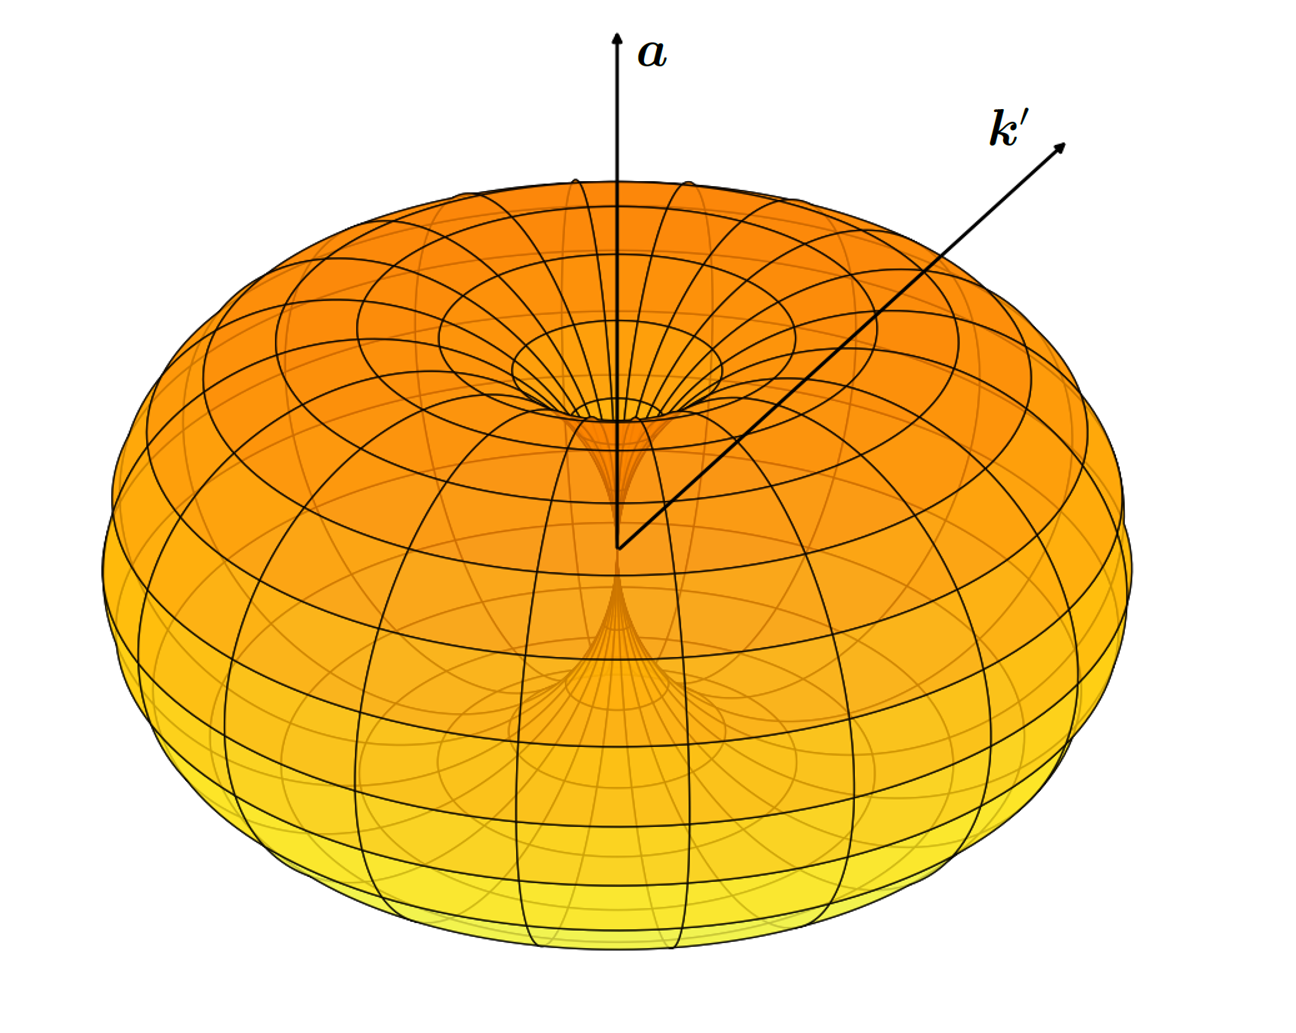
\includegraphics[scale=0.5]{Appendix-C/Figures/torus_radiation_edit.png}
 \caption[Characteristic torus shape of electric dipole radiation in coherent scattering]{Characteristic $\sin^2 \left( \vartheta \right)$ torus shape of Larmor radiation, where $\vartheta$ is the angle between the charge acceleration $\mathbold{a}$ and the propagation direction of scattered ray, which is represented by $\mathbold{k}'$.}\label{fig:torus_radition} 
 \end{figure} 
The toroidal shape seen in \cref{fig:torus_radition} represents the magnitude of the radiated intensity, which depends on $E^2_{\text{rad}} \left( R, t \right)$ and hence is proportional to $\sin^2 \left( \vartheta \right)$. 

The above scenario outlines the process of Thomson scattering for a single electron from a classical viewpoint: an incident electromagnetic wave of frequency $\omega$ induces the charge to oscillate, which in turn produces radiation of the same frequency in a characteristic toroidal pattern. 
From a quantum-mechanical perspective, the distribution seen in \cref{fig:torus_radition} represents the probability for a single photon to be scattered in a particular direction defined by $\mathbold{k}'$ \cite{Shankar04,deBergevin09,Attwood17,Als-Nielsen11}. 
However, because the approximation $\mathcal{E}_{\gamma} \gg \mathcal{E}_e$ is generally not valid for soft x-rays, restoring and damping forces for atomic electrons must be taken into account. 
That is, in analogy to the concept of vibrational resonance in a macroscopic object, the $j^{\text{th}}$ electron in an atom can be thought of semi-classically as having a resonance frequency, $\omega_j$, that it is equivalent to $\omega_e \equiv \mathcal{E}_{e} / \hbar$ introduced at the start of \cref{sec:SXR_med}. 
Simultaneously, the oscillation is damped as the electron radiates away its energy from a classical perspective; this is accounted for with a damping term, $\Gamma_j$.\footnote{Quantum-mechanically, $\Gamma_j$ is associated with the transition rate [\emph{cf.\@} \cref{sec:transition_rate_sub}] and hence damping of the probability for a scattering event to occur, which ultimately results in a small spread of possible energies for the scattered photon. 
That is, in a similar manner to the damping behavior exhibited in bound-bound transitions that result in naturally-broadened spectral lines [\emph{cf.\@} \cref{sec:form_spectral}], $\Gamma_j$ characterizes the width of this distribution, which can be assumed to be very small such that $\Gamma_j \ll \omega$.} 
While determining values for $\omega_j$ and $\Gamma_j$ from theory requires the use of rigorous quantum mechanics, arguments familiar in classical physics in conjunction with tabulated data are sufficient to study how coherent scattering depends on $\omega$ and the particular type of atom under question \cite{Shankar04,deBergevin09,Attwood17,Als-Nielsen11}. 

With knowledge of the range of binding frequencies, $\omega_j$, for the elements and the assumption that $\Gamma_j / \omega \ll 1$, coherent scattering that takes into account atomic resonances can be treated under the Born approximation framework discussed above \cite{Attwood17,deBergevin09}.  
However, unlike relatively long-$\lambda$ radiation such as visible light, $\lambda$ for soft x-rays is comparable to the spatial distribution of electrons in an atom as alluded to previously. 
Because of this, each of the $\mathcal{Z}$ electrons in an atom generally experiences a different phase of the incident wave, which affects how each electron oscillates about its average position, $\Delta \mathbold{r}_j$, and in turn, the overall scattering event. 
Illustrated for a single electron in \cref{fig:atomic_scattering}, this vector $\Delta \mathbold{r}_j$ originates at the location of the atomic nucleus while the oscillation is described by some function $\mathbold{X}_j (t)$, which is to be determined. 
\begin{figure}
 \centering
 \includegraphics[scale=1.25]{Appendix-C/Figures/scattering1.mps}
 \caption{Coherent scattering from the $j^{\text{th}}$ electron in a neutral atom with $\mathcal{Z}$ electrons}\label{fig:atomic_scattering}
 \end{figure}
The electric field felt by the $j^{\text{th}}$ electron then is $\mathbold{E}_j(\Delta \mathbold{r}_j,t) = \mathbold{E}_{0} \mathrm{e}^{i \left( \mathbold{k} \cdot \Delta \mathbold{r}_j - \omega t \right)}$ and therefore each electron in general radiates with a different phase as observed in the far-field. 
As a generalization of \cref{eq:acceleration_electron}, equating forces gives the following differential equation that describes the position $\mathbold{X}_j (t)$ of the $j^{\text{th}}$ electron \cite{Attwood17,deBergevin09}: 
\begin{subequations}
\begin{equation}\label{eq:osc_diff_eq}
 \dv[2]{\mathbold{X}_j (t)}{t} + \Gamma_j \dv{\mathbold{X}_j (t)}{t} + \omega_j^2 \mathbold{X}_j (t) = - \frac{q_e}{m_e} \mathbold{E}_0 \mathrm{e}^{i \left( \mathbold{k} \cdot \Delta \mathbold{r}_j - \omega t \right)} .
 \end{equation}
With the assumption that $v=|\mathbold{v}| \ll c_0$ for non-relativistic atomic electrons stated at the start of \cref{sec:SXR_med}, the position of each electron is considered to oscillate about $\Delta \mathbold{r}_j$ with the same time dependence of the driving field: $\mathbold{X}_j (t) = \Delta \mathbold{X}_j \mathrm{e}^{-i \omega t}$. 
Factors of $\mathrm{e}^{-i \omega t}$ drop out when this is inserted into \cref{eq:osc_diff_eq} and solving for the oscillation amplitude $\Delta \mathbold{X}_j$ gives \cite{Attwood17,deBergevin09}:
\begin{equation}\label{eq:electron_osc_amp}
 \Delta \mathbold{X}_j \equiv \frac{\mathbold{X}_j (t)}{\mathrm{e}^{-i \omega t}} = \frac{q_e}{m_e} \frac{\mathbold{E}_0 \mathrm{e}^{i \mathbold{k} \cdot \Delta \mathbold{r}_j}}{\left( \omega^2 - \omega_j^2 + i \omega \Gamma_j \right)} . 
 \end{equation}
\end{subequations}

For a point of observation $\mathbold{r}$,\footnote{To clarify, this is an arbitrary position in the line of sight for a scattered wave (given by $\mathbold{k}'$), where the electric field radiated by the atomic electrons is supposed to be measured.} the distance from the $j^{\text{th}}$ electron is $R_j \equiv | \mathbold{r} -\Delta \mathbold{r}_j |$ and the magnitude of the radiated electric field in the far-field (\emph{i.e.}, $R_j \gg c_0 / \omega$) is
%\begin{subequations}
\begin{equation}\label{eq:single_electron_radiate}
 E_{\text{rad},j} \left( R_j, t \right) = \frac{q_e \sin \left( \vartheta \right)}{4 \pi \epsilon_0 c_0^2 R_j} \dv[2]{X_j (t - R_j/c_0)}{t} = - \frac{q_e \omega^2 \sin \left( \vartheta \right)}{4 \pi \epsilon_0 c_0^2} \frac{\abs{\Delta \mathbold{X}_j} \mathrm{e}^{i \omega \left( \frac{R_j}{c_0} - t \right)}}{R_j} ,
 \end{equation}
where $X_j (t) \equiv \abs{\mathbold{X}_j (t)}$ and $\vartheta$ is the angle between the direction of charge oscillation along $\mathbold{E}_0$ and the direction of the outgoing scattered wave denoted by $\mathbold{k}'$ [\emph{cf.\@} \cref{fig:atomic_radiating}]. 
\begin{figure}
 \centering
 \includegraphics[scale=1.25]{Appendix-C/Figures/scattering3.mps}
 \caption[Scattering geometry for the $j^{\text{th}}$ electron in an atom]{Scattering geometry for the $j^{\text{th}}$ electron in an atom that oscillates along a direction defined by $\Delta \mathbold{X}_j$, which is parallel to the electric field of the incident electromagnetic wave with vector amplitude $\mathbold{E}_0$ (and perpendicular to the magnetic field with vector amplitude $\mathbold{H}_0$, as in \cref{fig:wavefront}). By \cref{eq:single_electron_radiate}, the magnitude of the radiated electric field (at a far-field distance from the electron $R_j$) depends on the angle $\vartheta$.}\label{fig:atomic_radiating}
 \end{figure} 
The magnitude of the radiated electric field at a far-field position $\mathbold{r}$ for an atom with $\mathcal{Z}$ electrons then is
\begin{align}
 \begin{split} \label{eq:charge_radiation1}
 E_{\text{rad}} \left( \mathbold{r} , t \right) &= \sum_{j=1}^{\mathcal{Z}} E_{\text{rad},j} \left( R_j, t \right) = - \frac{q_e \omega^2 \sin \left( \vartheta \right)}{4 \pi \epsilon_0 c_0^2} \mathrm{e}^{-i \omega t} \sum_{j=1}^{\mathcal{Z}} \frac{|\Delta \mathbold{X}_j|}{R_j} \mathrm{e}^{i k_0 R_j} \\
 &= - \abs{\mathbold{E}_0}  \mathrm{e}^{-i \omega t} r_e \sin \left( \vartheta \right) \sum_{j=1}^{\mathcal{Z}} \frac{\omega^2 \mathrm{e}^{i \left( k_0 R_j + \mathbold{k} \cdot \Delta \mathbold{r}_j \right)}}{R_j \left( \omega^2 - \omega_j^2 + i \omega \Gamma_j \right)} ,
 \end{split}
 \end{align} 
where \cref{eq:electron_osc_amp} was inserted for $\abs{\Delta \mathbold{X}_j}$ and $r_e \equiv q_e^2 / 4 \pi \epsilon_0 m_e c_0^2$ is the classical electron radius. 
For $\mathbold{r}$ with $\abs{\mathbold{r}} \equiv r \gg \abs{\Delta \mathbold{r}_j}$, the following approximations for $R_j \equiv | \mathbold{r} -\Delta \mathbold{r}_j |$ can be made: 
\begin{subequations}
\begin{equation}
 R_j^2 \approx r^2 - 2 \mathbold{r} \cdot \Delta \mathbold{r}_j \quad \text{and} \quad R_j \approx r \sqrt{\left( 1 - \frac{2 \mathbold{r} \cdot \Delta \mathbold{r}_j}{r^2} \right)} \approx r - \frac{\mathbold{r}}{r} \cdot \Delta \mathbold{r}_j 
 \end{equation}
and moreover, $\mathbold{r}/r$ is very close to the direction of the scattered wave given by $\mathbold{k}'/k_0$ such that the $R_j^{-1}$ term in \cref{eq:charge_radiation1} is roughly equal to $r^{-1}$ \cite{Attwood17}. 
Then, 
\begin{equation}
 k_0 R_j \approx k_0 \left( r - \frac{\mathbold{r}}{r} \cdot \Delta \mathbold{r}_j \right) \approx k_0 r - \mathbold{k}' \cdot \Delta \mathbold{r}_j
 \end{equation}
\end{subequations}
and the term in the exponential of \cref{eq:charge_radiation1}, $k_0 R_j + \mathbold{k} \cdot \Delta \mathbold{r}_j$, can be approximated as $k_0 r + \mathbold{Q} \cdot \Delta \mathbold{r}_j$, with $\mathbold{Q} \equiv \mathbold{k} - \mathbold{k}'$ as the \emph{scattering vector}.\footnote{It may help to point out that this vector, also called the \emph{wave-vector transfer} \cite{deBergevin09,Als-Nielsen11} is sometimes defined with the opposite sign (\emph{i.e.}, $\mathbold{k}' - \mathbold{k}$) \cite{Landau60,Sinha88,deBergevin09,Attwood17} and written using other symbols such as $\mathbold{q}$ \cite{Landau60,Sinha88,deBergevin09} or $\Delta \mathbold{k}$ \cite{Attwood17}.} 
Finally, \cref{eq:charge_radiation1} becomes 
\begin{equation}\label{eq:charge_radiation2}
 E_{\text{rad}} \left( \mathbold{r} , t \right) = - \abs{\mathbold{E}_0}  \mathrm{e}^{i \left(k_0 r -\omega t \right)} \frac{r_e}{r} \sin \left( \vartheta \right) \sum_{j=1}^{\mathcal{Z}} \frac{\omega^2 \mathrm{e}^{i \mathbold{Q} \cdot \Delta \mathbold{r}_j}}{\left( \omega^2 - \omega_j^2 + i \omega \Gamma_j \right)} 
 \end{equation}
for a point of observation in the far-field, where $r \gg \abs{\Delta \mathbold{r}_j}$. 
%\end{subequations}

At this point, \cref{eq:charge_radiation2} describes the radiation produced from scattering in a single atom, where the spacing in between electrons cannot be neglected due to the condition $\lambda \gg a_0$ not being fulfilled. 
Dividing this expression by the magnitude of the incident electric field highlights the fact that the scattered field emerges as a spherical wavefront that is modulated by $\sin \left( \vartheta \right)$ and a complex function $f^a(\mathbold{Q},\omega)$ known as the \emph{atomic scattering factor} \cite{deBergevin09,Als-Nielsen11,Attwood17}: 
\begin{subequations}
\begin{equation}\label{eq:spherical_scatter}
 \frac{E_{\text{rad}} \left( \mathbold{r} , t \right)}{\abs{\mathbold{E}_0} \mathrm{e}^{-i \omega t}} = - r_e \sin \left( \vartheta \right) \left( \frac{\mathrm{e}^{i k_0 r}}{r} \right) f^a \left( \mathbold{Q}, \omega \right)  
 \end{equation}
with\footnote{This quantity can be formulated in a few different ways. In some texts \cite{deBergevin09,Als-Nielsen11}, a function of $\mathbold{Q}$ alone, referred to as the \emph{atomic structure factor}, is defined as the Fourier transform (with respect to $\mathbold{Q}$) of the electron distribution in an atom. Then, $\omega$-dependent (complex) dispersion corrections are introduced to account for the resonant behavior of bound electrons. These terms depending on $\mathbold{Q}$ and $\omega$ separately are added together to arrive at an expression for $f^a(\mathbold{Q},\omega)$, also called the \emph{atomic form factor}.} 
\begin{equation}\label{eq:atomic_scattering_factor}
 f^a \left( \mathbold{Q}, \omega \right) \equiv \sum_{j=1}^{\mathcal{Z}} \frac{\omega^2 \mathrm{e}^{i \mathbold{Q} \cdot \Delta \mathbold{r}_j}}{\left( \omega^2 - \omega_j^2 + i \omega \Gamma_j \right)} ,
 \end{equation} 
\end{subequations}
which describes how radiation of frequency $\omega$ is scattered by a particular type of atom in a direction given by the scattering vector, $\mathbold{Q}$. 
Using the scattering angle defined in \cref{fig:atomic_scattering}, $\theta_{sc}$, the magnitude of this vector is
\begin{subequations}
\begin{equation}\label{eq:scattering_angle}
 \abs{\mathbold{Q}} \equiv \abs{\mathbold{k} - \mathbold{k}'} = 2 k_0 \sin \left( \theta_{sc} \right) = \frac{4 \pi}{\lambda} \sin \left( \theta_{sc} \right) 
 \end{equation}
and assuming $\abs{\Delta \mathbold{r}_j} \sim a_0$, the phase term $\mathbold{Q} \cdot \Delta \mathbold{r}_j$ in \cref{eq:charge_radiation2,eq:atomic_scattering_factor} has a magnitude bounded by 
\begin{equation}\label{eq:atomic_phase_inequality}
 \abs{\mathbold{Q} \cdot \Delta \mathbold{r}_j} \leq \frac{4 \pi a_0}{\lambda} \sin \left( \theta_{sc} \right) . 
 \end{equation}
Therefore, the phase difference felt by each of the $j$ electrons can be ignored when the following condition is met \cite{Attwood17}: 
\begin{equation}\label{eq:scatter_condition}
 \sin \left( \theta_{sc} \right)  \ll \frac{\lambda}{a_0}, 
 \end{equation}
\end{subequations}
which occurs for near-forward scattering with $\mathbold{Q} \approx \mathbf{0}$ such that $f^a(\mathbold{Q},\omega)$ is at a maximum for a given $\omega$, where $\mathbf{0}$ is the null vector. 
Physically, this suggests that all electrons oscillate virtually in phase due to $\mathbold{k}$ and $\mathbold{k}'$ being close to parallel. 
In contrast, $f^a(\mathbold{Q},\omega)$ decreases with increasing $\mathbold{Q}$ and these scattered waves of different phases tend to cancel each other out \cite{Als-Nielsen11}. 

For radiation with $\lambda \lessapprox a_0$, \cref{eq:scatter_condition} is only satisfied for a particular range of $\theta_{sc}$. 
Hard x-rays with large $a_0 / \lambda$, for example, only meet this condition for very small $\theta_{sc}$. 
However, as $\lambda$ becomes large compared to $a_0$ (\emph{e.g.}, the red end of the soft x-ray spectrum), this condition for $\theta_{sc}$ is loosened and as a result, scattering with all electrons in phase can occur over a slightly wider range of angles \cite{Attwood17}. %double-check this...
As $\lambda$ increases further to the point of becoming characteristic of visible light, $a_0 / \lambda$ is very small and thus coherent scattering occurs over all angles. 
For any of these cases, \cref{eq:atomic_scattering_factor} can be simplified to:
\begin{equation}\label{eq:atomic_scattering_factor_reduced1}
 f^a \left( \mathbf{0}, \omega \right) \equiv f^0 \left( \omega \right) = \sum_{j=1}^{\mathcal{Z}} \frac{\omega^2}{\left( \omega^2 - \omega_j^2 + i \omega \Gamma_j \right)} , 
 \end{equation}
where the superscript$^0$ indicates that the \emph{forward-scattering approximation} with $\mathbold{Q} \to \mathbf{0}$ has been made \cite{Attwood17}. 

Equivalently, $f^0 \left( \omega \right)$ can be defined using scattering \emph{oscillator strengths} denoted by $g_s$, which can loosely be understood as the number electrons with a binding frequency $\omega_s$ with $\sum_s g_s = \mathcal{Z}$:\footnote{Quantum-mechanically, $g_s$ for a given atomic scattering event is related to the transition rate, $\Gamma$, while $\sum_s g_s = \mathcal{Z}$ follows from the \emph{Thomas-Reiche-Kuhn sum rule} \cite{Attwood17,Rybicki86}.}
\begin{subequations}
\begin{equation}\label{eq:atomic_scattering_factor_reduced2}
 f^0 \left( \omega \right) \equiv \sum_s \frac{g_s \, \omega^2}{\left( \omega^2 - \omega_s^2 + i \omega \Gamma_s \right)} .
 \end{equation} 
This quantity is directly related to the effective scattering cross-section for radiation of frequency $\omega$ \cite{Als-Nielsen11,Attwood17}:
\begin{equation}\label{eq:scattering_cross-section}
 \sigma_a \left( \omega \right) = \frac{8 \pi}{3} r_e^2 \, \norm{f^0 \left( \omega \right)}^2 = \sigma_e \, \norm{\sum_s \frac{g_s \omega^2}{\left( \omega^2 - \omega_s^2 + i \omega \Gamma_s \right)}}^2 ,
 \end{equation}
where $\sigma_e \equiv 8 \pi r_e^2 / 3$ is the \emph{Thomson cross-section} for a free electron. 
Note that for a scenario where $\omega$ is much higher than all $\omega_s$ in a particular atom, $f^0(\omega) \to \mathcal{Z}$ and $\sigma_a \left( \omega \right) \to \mathcal{Z}^2 \sigma_e$, which is characteristic of Thomson scattering for $\mathcal{Z}$ electrons. 
Mentioned previously, hard x-rays scattering from electrons in relatively light atoms can be described in this way while on the other hand, the opposite case with $\omega \ll \omega_s$ has \cref{eq:scattering_cross-section} reducing to the well-known expression for the Rayleigh scattering cross-section
\begin{equation}
 \sigma_a \left( \omega \right) \to \sigma_e \sum_s g_s^2 \left( \frac{\omega}{\omega_s} \right)^{4} ,
 \end{equation}
\end{subequations}
which indicates that the amplitude of scattering by a single bound electron has a $\omega^4$ dependence \cite{Jackson75,deBergevin09,Attwood17}. 

Complex atomic scattering factors in the forward-scattering approximation, $f^0(\omega)$, are plotted as a function of photon energy $\mathcal{E}_{\gamma} = \hbar \omega$ across the soft x-ray spectrum in \cref{fig:atomic_scattering_data,fig:atomic_scattering_data2,fig:atomic_scattering_data3} for a few light elements using data tabulated by the Center for X-ray Optics (CXRO) at Lawrence Berkeley National Laboratory \cite{CXRO_database,LBNL_web}. 
\begin{figure}
 \centering
 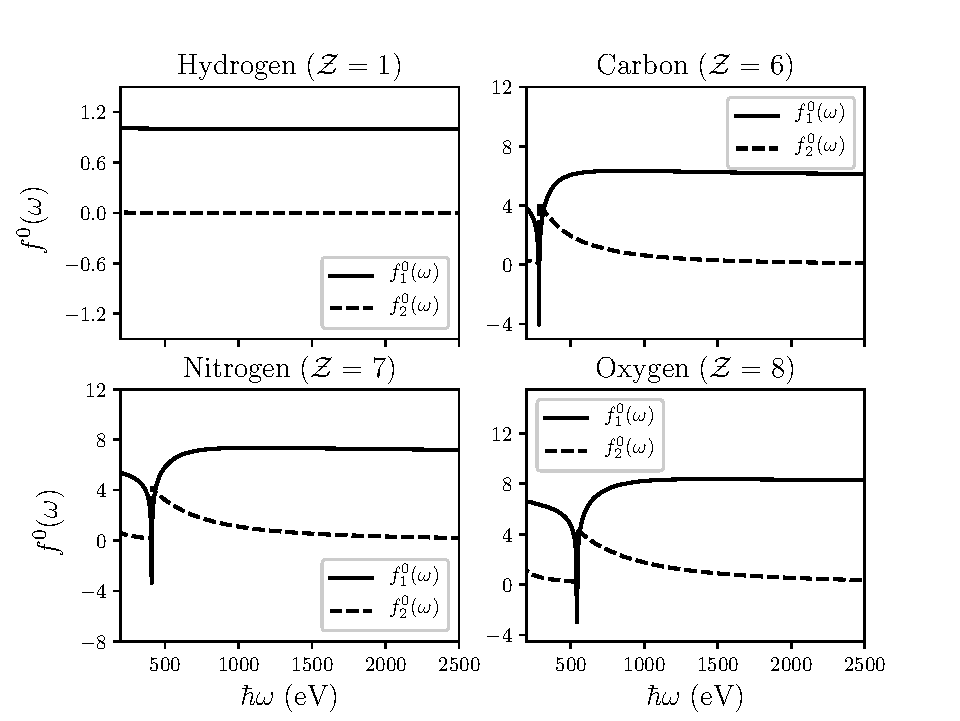
\includegraphics[scale=0.95]{Appendix-C/Figures/atomic_scattering_factor.pdf}
 \caption[Atomic scattering factors for hydrogen, carbon, nitrogen and oxygen across the soft x-ray spectrum]{Atomic scattering factors for hydrogen, carbon, nitrogen and oxygen in the forward-scattering approximation across the soft x-ray spectrum \cite{CXRO_database}}\label{fig:atomic_scattering_data}
 \end{figure}
\begin{figure}
 \centering
 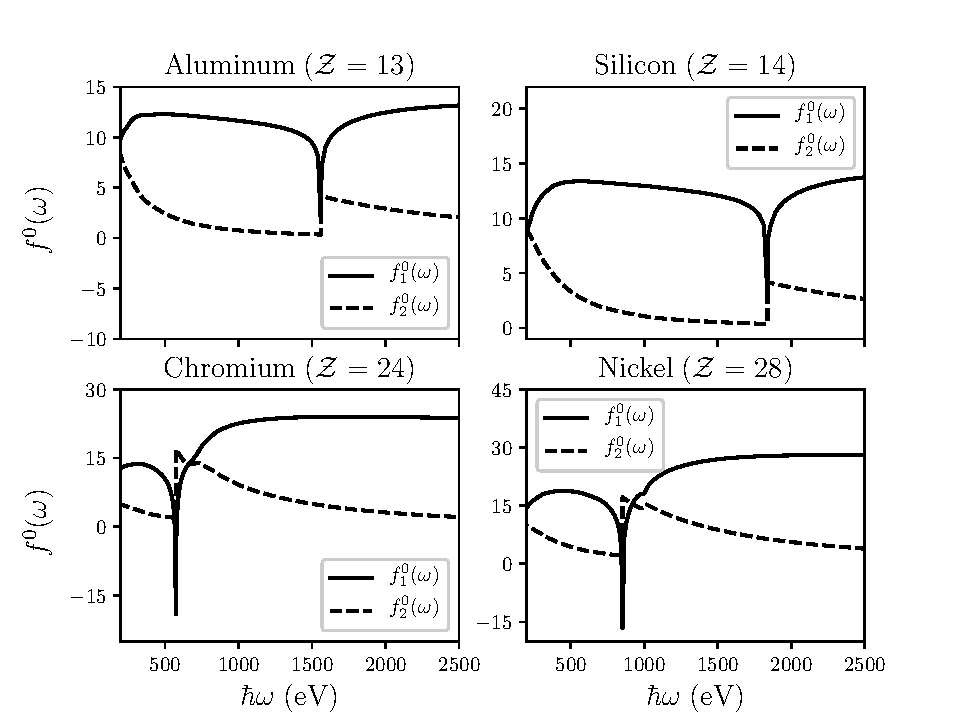
\includegraphics[scale=0.95]{Appendix-C/Figures/atomic_scattering_factor_2.pdf}
 \caption[Atomic scattering factors for aluminum, silicon, chromium and nickel across the soft x-ray spectrum]{Atomic scattering factors for aluminum, silicon, chromium and nickel in the forward-scattering approximation across the soft x-ray spectrum \cite{CXRO_database}}\label{fig:atomic_scattering_data2}
 \end{figure}
\begin{figure}
 \centering
 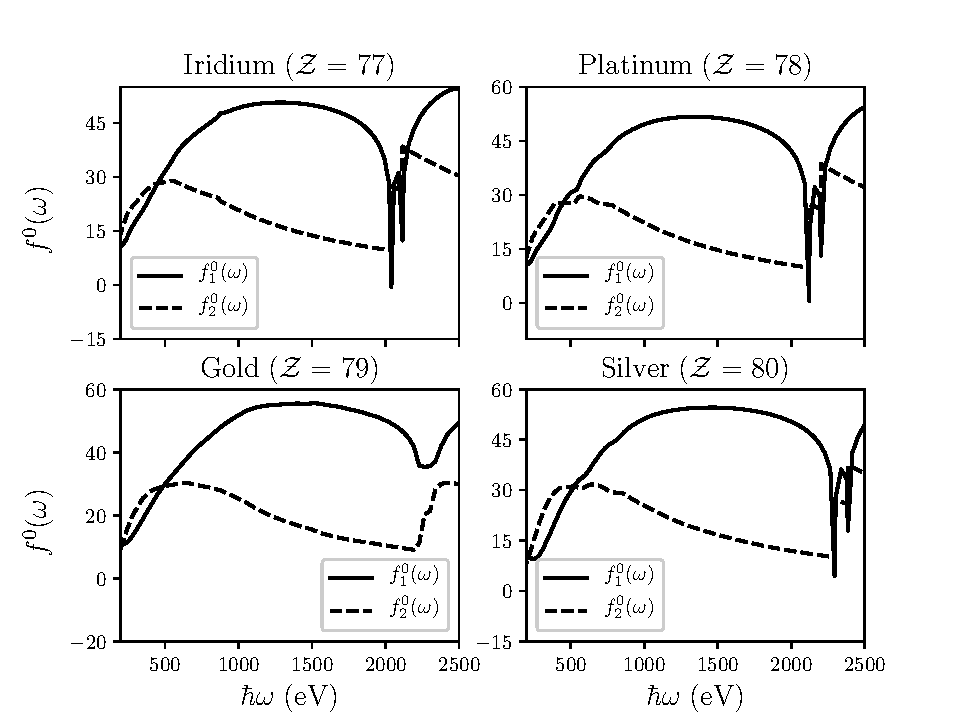
\includegraphics[scale=0.95]{Appendix-C/Figures/atomic_scattering_factor_3.pdf}
 \caption[Atomic scattering factors for iridium, platinum, gold and silver across the soft x-ray spectrum]{Atomic scattering factors for iridium, platinum, gold and silver in the forward-scattering approximation across the soft x-ray spectrum \cite{CXRO_database}}\label{fig:atomic_scattering_data3}
 \end{figure}
In the plots, $f^0(\omega)$ is decomposed into real and imaginary parts: 
\begin{equation}\label{eq:atomic_scattering_factor_reduced3}
 f^0 \left( \omega \right) = \Re \left[ f^0 \left( \omega \right) \right] + i \Im \left[ f^0 \left( \omega \right) \right] \equiv f_1^0 \left( \omega \right) - i f_2^0 \left( \omega \right) ,
 \end{equation} 
where $f_1^0(\omega)$ is associated with the amplitude of the scattered wave while $f_2^0(\omega)$ is related to attenuation and absorption. 
As can be gleaned from these figures, $f_1^0(\omega)$ tends to increase with $\mathcal{Z}$, which represents the number of electrons that are radiating together in phase under the forward-scattering approximation. 
Meanwhile, $f_2^0(\omega)$ also increases with $\mathcal{Z}$, where the effect is most pronounced near prominent \emph{absorption edges} that are caused by photo-ionization. 

K-shell absorption edges are seen clearly in \cref{fig:atomic_scattering_data} for carbon, nitrogen and oxygen ($\mathcal{Z}=$ \numrange{6}{8}) whereas there is a flat response from the lone electron in hydrogen ($\mathcal{Z}=1$) that has $\mathcal{E}_e \approx \SI{13.6}{\electronvolt}$, which is much smaller than $\mathcal{E}_{\gamma} \equiv \hbar \omega$ for soft x-rays.
As a result, soft x-rays experience a high degree of absorption and attenuation in the elements with $\mathcal{Z} \geq 6$ while on the other hand, hydrogen and other very light elements are virtually transparent to soft x-rays with $f_1^0(\omega) \approx 1$ and $f_2^0(\omega)$ not departing significantly from zero, which is analogous to the behavior exhibited by hard x-rays scattering from low-to-mid $\mathcal{Z}$ atoms. 
Further, \cref{fig:atomic_scattering_data2} shows higher-energy K-shell absorption edges in aluminum and silicon ($\mathcal{Z}=$ \numlist{13;14}) while L-shell absorption lines at lower $\mathcal{E}_{\gamma}$ are seen in chromium and nickel ($\mathcal{Z}=$ \numlist{24;28}).\footnote{Note, however, that each of these four atoms tend to bond with oxygen so that in practice, these materials oxidize and hence some degree of oxygen absorption should also be expected.}
Although relativistic corrections are needed to treat scattering from high-$\mathcal{Z}$ atoms such as iridium, platinum, gold and silver ($\mathcal{Z}=$ \numrange{77}{80}), experimentally-determined values\footnote{CXRO tabulates data for chemical elements up to uranium ($\mathcal{Z} = 92$) \cite{Henke93,Gullikson98,CXRO_database,Attwood17}. In practice, $f_2^0(\omega)$ is experimentally determined by measuring absorption while $f_1^0(\omega)$ follows from the \emph{Kramers-Kronig relations} for causal consistency \cite{Kronig26,Als-Nielsen11,Attwood17,Jackson75,Landau60}.} of $f_1^0(\omega)$ and $f_2^0(\omega)$ for these atoms are plotted in \cref{fig:atomic_scattering_data3}. 
Signatures of M-shell absorption in these heavy atoms are seen at $\mathcal{E}_{\gamma} > \SI{2}{\kilo\electronvolt}$ while N-shell absorption contributes to attenuation for $\mathcal{E}_{\gamma} \lessapprox \SI{800}{\electronvolt}$. 
Due to this broadband response free of sharp absorption edges below \SI{2}{\kilo\electronvolt}, these materials are desirable for soft x-ray reflectivity; this is discussed further in the next section. %\cref{sec:x-ray_index}. 

\subsection{Soft X-ray Index of Refraction}\label{sec:x-ray_index}
%%%%%%%%%%%%%%%%%%%%%%%%%%%%%%%%%%%%%%%%%--------------------------------------------------
Typically, the \emph{index of refraction} of a material is defined macroscopically for radiation of a given frequency $\omega$ assuming $\lambda \gg a_0$. 
For visible light, where $\omega$ is large enough to neglect contributions from magnetic-dipole interactions as discussed at the start of \cref{sec:SXR_med}, the index of refraction depends only on the electric polarization field, $\mathbold{P}(\mathbold{r},t)$ [\emph{cf.\@} \cref{eq:electric_polarization_field}], as it enters through the \emph{electric displacement field}, $\mathbold{D}(\mathbold{r},t)$, which is defined as \cite{Landau60,Jackson75,Griffiths17,Born80}: 
\begin{subequations}
\begin{equation}\label{eq:displacement_field_def}
 \mathbold{D}(\mathbold{r},t) \equiv \epsilon_0 \mathbold{E}(\mathbold{r},t) + \mathbold{P}(\mathbold{r},t) .
 \end{equation}
Because it takes a finite amount of time for atomic electric-dipole moments to respond to $\mathbold{E}(\mathbold{r},t)$, $\mathbold{D}(\mathbold{r},t)$ depends on $\mathbold{E}(\mathbold{r},t)$ not only at a time $t$ like it does in quasi-static situations,\footnote{For example, in electrostatics and in situations where $\mathbold{E}(\mathbold{r},t)$ varies slowly in time, the relation $\mathbold{D}(\mathbold{r},t) = \epsilon \mathbold{E}(\mathbold{r},t)$ (with $\epsilon$ as a constant) can often be used.} but also generally on all previous times leading up to $t$. 
This can be written as:%define linear material
\begin{equation}
 \mathbold{D}(\mathbold{r},t) = \epsilon_0 \mathbold{E}(\mathbold{r},t) + \int_0^{\infty} f_{\epsilon} (t') \, \mathbold{E}(\mathbold{r},t-t') \dd{t'} ,
 \end{equation}
where $f_{\epsilon} (t')$ is, for now, an unknown function of time that depends on the properties of a given material \cite{Landau60,Jackson75}. 
Expressing the fields as inverse Fourier transforms shows that $\mathbold{D}(\mathbold{r},t)$ and $\mathbold{E}(\mathbold{r},t)$ are related to each other through a complex, material-dependent function of frequency:
\begin{align}
 \begin{split}\label{eq:epsilon_omega_def}
 \mathbold{D}(\mathbold{r},t) &= \frac{1}{2 \pi} \int_{-\infty}^{\infty} \mathbold{D}(\mathbold{r},\omega) \, \mathrm{e}^{-i \omega t} \dd{\omega} \\
 &= \frac{\epsilon_0}{2 \pi} \int_{-\infty}^{\infty} \mathbold{E}(\mathbold{r},\omega) \, \mathrm{e}^{-i \omega t} \dd{\omega} + \frac{1}{2 \pi} \int_{-\infty}^{\infty} \int_{0}^{\infty} f_{\epsilon} (t') \, \mathrm{e}^{-i \omega (t - t')} \mathbold{E}(\mathbold{r},\omega) \dd{t'} \dd{\omega} \\
 &= \left[ \epsilon_0 + \int_{0}^{\infty} f_{\epsilon} (t') \, \mathrm{e}^{i \omega t'} \dd{t'} \right] \mathbold{E}(\mathbold{r},t) \equiv \epsilon (\omega) \, \mathbold{E}(\mathbold{r},t) . %\\ %&\quad \quad \quad
 \end{split}
 \end{align}
\end{subequations}
Using this function $\epsilon (\omega)$, which describes permittivity of the medium for a given frequency, the complex index of refraction is defined as 
\begin{equation}\label{eq:refractive_index}
 \tilde{\nu} (\omega) \equiv \sqrt{\frac{\epsilon (\omega)}{\epsilon_0}} .
 \end{equation}
However, as emphasized in the preceding discussion, the condition $\lambda \gg a_0$ is not fulfilled for soft x-rays. 
Notwithstanding this, an effective index of refraction can be formulated by using an approximate expression for $\mathbold{P}(\mathbold{r},t)$ that takes into account the density of atoms constituting a material. 

In principle, describing the behavior of soft x-rays in a medium requires solving the microscopic form of Maxwell's equations [\emph{cf.\@} \cref{eq:Maxwell_vac_start_1,eq:Maxwell_vac_start_2,eq:Maxwell_vac_start_3,eq:Maxwell_vac_start_4}] using the electric charge and current present in individual atoms as source terms \cite{Attwood17,deBergevin09}. 
On the other hand, the macroscopic version of Maxwell's equations in a dispersive medium can be expressed in a time-harmonic form similar to \cref{eq:Maxwell_vac_TH_1,eq:Maxwell_vac_TH_2,eq:Maxwell_vac_TH_3,eq:Maxwell_vac_TH_4} for electromagnetic waves in vacuum. 
In the absence of free charge and current, these can be written as:
\begin{subequations}
\begin{align} 
 \mathbold{\nabla} \cdot \mathbold{E} \left( \mathbold{r} \right) &= 0 \label{eq:Maxwell_med_TH_1} \\
 \mathbold{\nabla} \cdot \mathbold{H} \left( \mathbold{r} \right) &= 0 \label{eq:Maxwell_med_TH_2} \\
 \mathbold{\nabla} \times \mathbold{E} \left( \mathbold{r} \right) &= i \omega \mu_0 \mathbold{H} \left( \mathbold{r} \right) \label{eq:Maxwell_med_TH_3} \\
 \mathbold{\nabla} \times \mathbold{H} \left( \mathbold{r} \right) &= -i \omega \epsilon (\omega) \mathbold{E} \left( \mathbold{r} \right) \label{eq:Maxwell_med_TH_4} ,
 \end{align}
\end{subequations}
with $\mu_0$ as the vacuum permeability. 
These equations can be rearranged\footnote{That is, by taking curls of \cref{eq:Maxwell_med_TH_3,eq:Maxwell_med_TH_4}: 
\begin{align*}
 \begin{split}
 \mathbold{\nabla} \times \mathbold{\nabla} \times \mathbold{E}(\mathbold{r}) &= \mathbold{\nabla}\left[\mathbold{\nabla} \cdot \mathbold{E}(\mathbold{r})\right] - \laplacian \mathbold{E}(\mathbold{r}) = i \omega \mu_0 \mathbold{\nabla} \times \mathbold{H} (\mathbold{r}) = \mu_0 \epsilon (\omega) \omega^2 \mathbold{E} (\mathbold{r}) \\
 \mathbold{\nabla} \times \mathbold{\nabla} \times \mathbold{H}(\mathbold{r}) &= \mathbold{\nabla}\left[\mathbold{\nabla} \cdot \mathbold{H}(\mathbold{r})\right] - \laplacian \mathbold{H}(\mathbold{r}) = - i \epsilon (\omega) \mathbold{\nabla} \times \mathbold{E} (\mathbold{r}) = \mu_0 \epsilon (\omega) \omega^2 \mathbold{H} (\mathbold{r})
 \end{split}
 \end{align*}
and inserting \cref{eq:Maxwell_med_TH_1,eq:Maxwell_med_TH_2}.} to give the following expression: 
\begin{equation} \label{eq:Helmholtz_med}
 \left( \laplacian + \mu_0 \epsilon (\omega) \omega^2 \right) \left\{
  \begin{array}{lr}
  \mathbold{E}(\mathbold{r})\\
  \mathbold{H}(\mathbold{r})
  \end{array}
 \right\} = \mathbf{0} ,
 \end{equation}
which is recognized as the \emph{Helmholtz equation} for the medium \cite{Landau60,Jackson75}. 
Similar to what is done in \cref{sec:EM_waves_vac} for electromagnetic waves in vacuum, solutions to \cref{eq:Helmholtz_med} can be studied by expressing the time-harmonic fields as a superposition of spatial wave modes using inverse Fourier transforms:
\begin{equation} \label{eq:fourier_fields_complex}
 \left\{
  \begin{array}{lr}
  \mathbold{E} \left( \mathbold{r} \right) \\
  \mathbold{H} \left( \mathbold{r} \right)
  \end{array}
 \right\} = \frac{1}{(2 \pi)^3} \int_{-\mathbold{\infty}}^{\mathbold{\infty}} \left\{
  \begin{array}{lr}
  \mathbold{E} \left( \mathbold{\tilde{k}} \right) \\
  \mathbold{H} \left( \mathbold{\tilde{k}} \right)
  \end{array}
 \right\} \mathrm{e}^{i \mathbold{\tilde{k}} \cdot \mathbold{r}} \dd[3]{\mathbold{\tilde{k}}},
 \end{equation}
where $\mathbold{\tilde{k}}$ is a wave vector that characterizes the direction of wave propagation and the spatial frequency of the electromagnetic fields.

Because $\epsilon(\omega)$ is generally complex, $\mathbold{\tilde{k}}$ is considered to be a complex wave vector:
%\begin{subequations}
\begin{equation}
 \mathbold{\tilde{k}} = \mathbold{k} + i \mathbold{\kappa} , \label{eq:k_tilde_def}
 \end{equation}
where $\mathbold{k}$ and $\mathbold{\kappa}$ are real vectors denoting the direction and magnitude of wave propagation and wave attenuation, respectively. 
Inserting \cref{eq:fourier_fields_complex} into \cref{eq:Helmholtz_med} gives 
\begin{equation}
 \laplacian \left\{
  \begin{array}{lr}
  \mathbold{E} \left( \mathbold{r} \right) \\
  \mathbold{H} \left( \mathbold{r} \right)
  \end{array}
 \right\} = \frac{1}{(2 \pi)^3} \laplacian \int_{-\mathbold{\infty}}^{\mathbold{\infty}} \left\{
  \begin{array}{lr}
  \mathbold{E} \left( \mathbold{\tilde{k}} \right) \\
  \mathbold{H} \left( \mathbold{\tilde{k}} \right)
  \end{array}
 \right\} \mathrm{e}^{i \mathbold{\tilde{k}} \cdot \mathbold{r}} \dd[3]{\mathbold{\tilde{k}}}
  = - \tilde{k}^2 \left\{
  \begin{array}{lr}
  \mathbold{E} \left( \mathbold{r} \right) \\
  \mathbold{H} \left( \mathbold{r} \right)
  \end{array}
 \right\} 
 \end{equation}
with
\begin{equation}\label{eq:disp_rel_med}
 \tilde{k}^2 \equiv \mathbold{\tilde{k}} \cdot \mathbold{\tilde{k}} = \mathbold{k} \cdot \mathbold{k} + 2 i \mathbold{k} \cdot \mathbold{\kappa} - \mathbold{\kappa} \cdot \mathbold{\kappa} = \mu_0 \, \epsilon (\omega) \, \omega^2 
 \end{equation}
%\end{subequations}
as the \emph{dispersion relation in the material}. 
Dividing this expression by $k_0^2 = \omega^2 \epsilon_0 \mu_0$ [\emph{cf.\@} \cref{eq:disp_rel_vac}] shows that $\tilde{k} = k_0 \tilde{\nu} (\omega)$  while inserting \cref{eq:fourier_fields_complex} into \cref{eq:Maxwell_med_TH_1,eq:Maxwell_med_TH_2,eq:Maxwell_med_TH_3,eq:Maxwell_med_TH_4} yields the following expressions:
\begin{subequations}
\begin{align} %eq:Maxwell_med_TH 1-4
 \left( \mathbold{k} + i \mathbold{\kappa} \right) \cdot \mathbold{E} \left( \mathbold{r} \right) &= 0 \label{eq:Maxwell_med_FT_1} \\
 \left( \mathbold{k} + i \mathbold{\kappa} \right) \cdot \mathbold{H} \left( \mathbold{r} \right) &= 0 \label{eq:Maxwell_med_FT_2} \\
 \left( \mathbold{k} + i \mathbold{\kappa} \right) \times \mathbold{E} \left( \mathbold{r} \right) &= Z_0 k_0 \mathbold{H} \left( \mathbold{r} \right) \label{eq:Maxwell_med_FT_3} \\
 \left( \mathbold{k} + i \mathbold{\kappa} \right) \times \mathbold{H} \left( \mathbold{r} \right) &= - \tilde{\nu}^2 (\omega) \frac{k_0}{Z_0} \mathbold{E} \left( \mathbold{r} \right) \label{eq:Maxwell_med_FT_4} ,
 \end{align}
\end{subequations}
with $Z_0$ as the impedance of free space. 
These equations indicate that, in contrast to the behavior of electromagnetic radiation in vacuum, the intensity of a wave drops off as $\mathrm{e}^{-2 \mathbold{\kappa} \cdot \mathbold{r}}$ as it propagates through a material and moreover, waves are only transverse in situations where $\mathbold{k}$ and $\mathbold{\kappa}$ are aligned; otherwise, wavefronts are distorted as they propagate and decay in different directions. 

Now, with $\lambda \gg a_0$ not fulfilled for soft x-rays, formulating $\tilde{\nu} (\omega)$ starts with considering the classical treatment of coherent scattering outlined in \cref{sec:scattering_atoms}, where the $j^{\text{th}}$ electron in an atom responds to an incident electromagnetic wave by oscillating about its average position, $\Delta \mathbold{r}_j$ [\emph{cf.\@} \cref{eq:osc_diff_eq,eq:electron_osc_amp}]. 
As this electrons oscillates along the direction of $\mathbold{E}_0$ with the function $\mathbold{X}_j (t) = \Delta \mathbold{X}_j \mathrm{e}^{-i \omega t}$ given by 
\begin{subequations}
\begin{equation}\label{eq:electron_osc}
 \mathbold{X}_j (t) = \frac{q_e}{m_e} \frac{\mathbold{E}_0 \mathrm{e}^{i \left( \mathbold{k} \cdot \Delta \mathbold{r}_j - \omega t \right)}}{\left( \omega^2 - \omega_j^2 + i \omega \Gamma_j \right)} ,
 \end{equation}
it radiates a wave of frequency $\omega$ according to \cref{eq:single_electron_radiate}. 
The most significant contributors to the modification of the incident wave, however, are forward-scattering events, where the phase term can be neglected [\emph{cf.\@} \cref{sec:scattering_atoms}]. 
In this case, each of the $\mathcal{Z}$ electrons in an atom oscillates in phase: 
\begin{equation}\label{eq:atomic_osc}
 \mathbold{X}_a (t) \equiv \sum_{j=1}^{\mathcal{Z}} \mathbold{X}_j (t) \approx \frac{q_e}{m_e} \mathbold{E}_0 \mathrm{e}^{-i \omega t} \underbrace{\sum_{s} \frac{g_s}{\left( \omega^2 - \omega_j^2 + i \omega \Gamma_j \right)}}_{f^0 (\omega) / \omega^2} ,
 \end{equation}
where $f^0 (\omega)$ is the atomic scattering factor in the forward-scattering approximation [\emph{cf.\@} \cref{eq:atomic_scattering_factor_reduced2}]. 
Therefore, the scattered intensity is at its maximum in this direction for a given $\omega$ as the atom behaves as a single, oscillating electric dipole:
\begin{equation}\label{eq:atomic_dipole_moment}
 \mathbold{p}_a (t) \equiv - q_e \mathbold{X}_a (t) .
 \end{equation}
\end{subequations}

For a large collection of atoms constituting a solid material with an average density of $\mathcal{N}_a$ atoms per unit volume, each atomic dipole is radiating its own wavefront but due to the relative positions of these atoms, partial destructive interference occurs unless the scattering angle illustrated in \cref{fig:atomic_scattering}, $\theta_{sc}$, is close to zero \cite{Attwood17}. 
In analogy with \cref{eq:atomic_phase_inequality}, this condition for $\theta_{sc}$ is approximately 
\begin{equation}
 \sin \left( \theta \right) \ll \frac{\lambda}{a} ,
 \end{equation}
where $a \equiv \mathcal{N}_a^{-1/3}$ is a typical spacing between atoms, which is usually several times larger than the Bohr radius, $a_0 \approx \SI{0.05}{\nm}$. 
Considering only scattered waves with $\theta_{sc} \to 0$ and a quasi-uniform medium with a near constant $\mathcal{N}_a$, \cref{eq:atomic_dipole_moment} can be used to express the electric polarization field as: 
\begin{equation}\label{eq:electric_polarization_model}
 \mathbold{P}(\mathbold{r},t) = - \mathcal{N}_a \frac{q_e^2}{m_e} \frac{f^0 (\omega)}{\omega^2} \mathbold{E} (\mathbold{r}, t) ,
 \end{equation}
where values for $\mathcal{N}_a$ for PMMA [\emph{cf.\@} \cref{sec:binary_ebeam}], silica (\ce{SiO2}), nickel and gold are listed in \cref{tab:element_densities}. 
\begin{table}[]
 \centering
 \caption[Mass density, atomic number density and typical atomic spacing for PMMA, silica, nickel and gold.]{Mass density, atomic number density and typical atomic spacing for PMMA (\ce{C5H8O2})$_n$, silica (\ce{SiO2}), nickel and gold \cite{CXRO_database}.}\label{tab:element_densities} 
 \begin{tabular}{@{}lllll@{}}
 \toprule  %calculated using CXRO value for g/cm^3 density, divided by the appropriate atomic mass (averages used for PMMA and silica)
 material & mass density & number density ($\mathcal{N}_a$) & typical atomic spacing \\ \midrule
 PMMA & \SI{1.19}{\gram\per\centi\metre\tothe{3}} & \num{1.08e29} atoms \si{\per\metre\tothe{3}} & $\mathcal{N}_a^{-1/3} \approx \SI{0.21}{\nm}$ \\ 
 silica & \SI{2.20}{\gram\per\centi\metre\tothe{3}} & \num{6.62e28} atoms \si{\per\metre\tothe{3}} & $\mathcal{N}_a^{-1/3} \approx \SI{0.25}{\nm}$ \\ 
 nickel & \SI{8.90}{\gram\per\centi\metre\tothe{3}} & \num{9.14e28} atoms \si{\per\metre\tothe{3}} & $\mathcal{N}_a^{-1/3} \approx \SI{0.22}{\nm} $\\ 
 gold & \SI{19.32}{\gram\per\centi\metre\tothe{3}} & \num{5.90e28} atoms \si{\per\metre\tothe{3}} & $\mathcal{N}_a^{-1/3} \approx \SI{0.27}{\nm}$ \\  \bottomrule
 \end{tabular}
 \end{table}
Then, using $\mathbold{P}(\mathbold{r},t) = \left[ \epsilon (\omega) - \epsilon_0  \right] \mathbold{E}(\mathbold{r},t)$ [\emph{cf.\@} \cref{eq:displacement_field_def,eq:epsilon_omega_def}] and $k_0^2 = \omega^2 / c_0^2 = (2 \pi / \lambda)^2$ [\emph{cf.\@} \cref{eq:disp_rel_vac}] yields the following expression for $\epsilon (\omega)$: % from \cref{eq:electric_polarization_model}:
\begin{equation}\label{eq:epsilon_omega_model}
 \epsilon (\omega)  = \epsilon_0 - \frac{\mathcal{N}_a q_e^2}{m_e} \frac{f^0 (\omega)}{\omega^2} = \epsilon_0 \left( 1 - \frac{4 \pi}{k_0^2} \mathcal{N}_a b^0 (\omega) \right) ,
 \end{equation}
where $b^0 (\omega) \equiv r_e f^0 (\omega)$ is the \emph{scattering length} in the forward-scattering approximation with $r_e \approx \SI{2.8e-15}{\metre}$ as the classical electron radius \cite{Als-Nielsen11,deBergevin09}.\footnote{In the limit of very high frequency, $\left( \omega^2 - \omega_s^2 + i \omega \Gamma_s \right) \approx \omega^2$ and therefore the electrons behave as if they were unbound and \cref{eq:epsilon_omega_model} becomes 
\begin{equation*}\label{eq:epsilon_omega_approx}
 \tilde{\nu}^2 (\omega) = \frac{\epsilon (\omega)}{\epsilon_0} \approx 1 - \frac{\omega_p^2}{\omega^2} \quad \text{with } \omega_p^2 \equiv \frac{\mathcal{N}_a \mathcal{Z} q_e^2}{\epsilon_0 m_e} ,
 \end{equation*}
where $\omega_p$ is the \emph{plasma frequency} of the medium. 
Physically, this reflects the fact that electron polarization processes cannot keep up when $\omega$ is sufficiently high, as alluded to previously \cite{Landau60,Jackson75}.} 

The complex index of refraction, which is valid for soft x-rays and other radiation satisfying the forward-scattering approximation can be expressed as [\emph{cf.\@} \cref{eq:refractive_index,eq:epsilon_omega_model}]
\begin{subequations}
\begin{equation}\label{eq:index_model}
 \tilde{\nu} (\omega) \equiv \left( \frac{\epsilon (\omega)}{\epsilon_0} \right)^{1/2} = \left( 1 - \frac{\lambda^2}{\pi} \mathcal{N}_a b^0 (\omega) \right)^{1/2} . 
 \end{equation}
From \cref{fig:atomic_scattering_data,fig:atomic_scattering_data2,fig:atomic_scattering_data3}, however, $\Re [b^0 (\omega)] \lessapprox 50 r_e \approx \SI{1.4e-13}{\metre}$ while, for soft x-rays, $\lambda^2 \sim \left( \SI{1}{\nm} \right)^2 = \SI{1e-18}{\metre\squared}$; with a typical value of $\mathcal{N}_a \sim \SI{e29}{\per\metre\tothe{3}}$ [\emph{cf.\@} \cref{tab:element_densities}], the quantity $\lambda^2 \mathcal{N}_a \Re \left[ b^0 (\omega) \right] / \pi$ is $\sim \num{e-3}$. 
Thus, it is justified to approximate \cref{eq:index_model} using the Taylor-series expansion of a square root, to first order:\footnote{\emph{i.e.}, $\sqrt{1 + x} \approx 1 + x/2$ for small $x$} 
\begin{equation}\label{eq:index_approx_alt}
 \tilde{\nu} (\omega) \approx \frac{\lambda^2}{2 \pi} \mathcal{N}_a b^0 (\omega) = 1 - 2 \pi \frac{c_0^2}{\omega^2} \mathcal{N}_a r_e f^0 (\omega) .
 \end{equation}
\end{subequations}
Similar to the treatment of $f^0 (\omega)$ in \cref{eq:atomic_scattering_factor_reduced3}, it is useful to split up $\tilde{\nu} (\omega)$ into real and imaginary components, $\nu(\omega)$ and $\xi(\omega)$, also known as the \emph{optical constants} [\emph{cf.\@} \cref{tab:optical_constants}]. 
\begin{table}[]
 \centering
 \caption[Notation for complex index of refraction]{Notation for complex index of refraction, $\tilde{\nu} (\omega)$}\label{tab:optical_constants}
 \begin{tabular}{@{}lll@{}} 
 \toprule
  & real part & imaginary part \\ \midrule
 this dissertation & $\nu (\omega) \equiv 1 - \delta_{\nu} (\omega)$  & $\xi (\omega)$ \\
 common optical notation  & $n$ & $k$ or $\kappa$ \\
 common x-ray notation & $1-\delta$ & $\beta$ \\ \bottomrule
 \end{tabular}
 \end{table}
This can be written as 
\begin{subequations}
\begin{equation}
 \tilde{\nu} (\omega) = \Re \left[ \tilde{\nu} (\omega) \right] + i \Im \left[ \tilde{\nu} (\omega) \right] \equiv \nu(\omega) + i \xi(\omega)
 \end{equation}
with 
\begin{align}
 \nu(\omega) &= 1 - 2 \pi \frac{c_0^2}{\omega^2} \mathcal{N}_a r_e f^0_1 \left( \omega \right) \equiv 1 - \delta_{\nu} (\omega) \quad \text{and} \\
 \xi(\omega) &= 2 \pi \frac{c_0^2}{\omega^2} \mathcal{N}_a r_e f^0_2 \left( \omega \right) ,
 \end{align}
where $f^0 \left( \omega \right) \equiv f^0_1 \left( \omega \right) - i f^0_2 \left( \omega \right)$ [\emph{cf.\@} \cref{eq:atomic_scattering_factor_reduced3}]. 
\end{subequations}
These expressions indicate that $\nu(\omega) < 1$ over the soft x-ray spectrum, with possible exceptions near resonances, where $\omega \approx \omega_s$. 
This implies that in an opposite fashion to visible light and other relatively long-$\lambda$ radiation, the phase velocity, $c_p \equiv c_0 / \nu (\omega)$, can be greater than $c_0$ for soft x-rays with the wavelength in the medium, $\lambda' \equiv \lambda / \nu(\omega)$, increasing relative to $\lambda$ rather than decreasing. 
Moreover, with $\nu(\omega) \lessapprox 1$, the effect refraction in the soft x-ray bandpass is expected to be small [\emph{cf.\@} \cref{sec:planar_interface}]. 

The optical constants defined above are plotted in \cref{fig:X-ray_index} for the materials listed in \cref{tab:element_densities} using data obtained from CXRO \cite{CXRO_database}. 
\begin{figure}
 \centering
 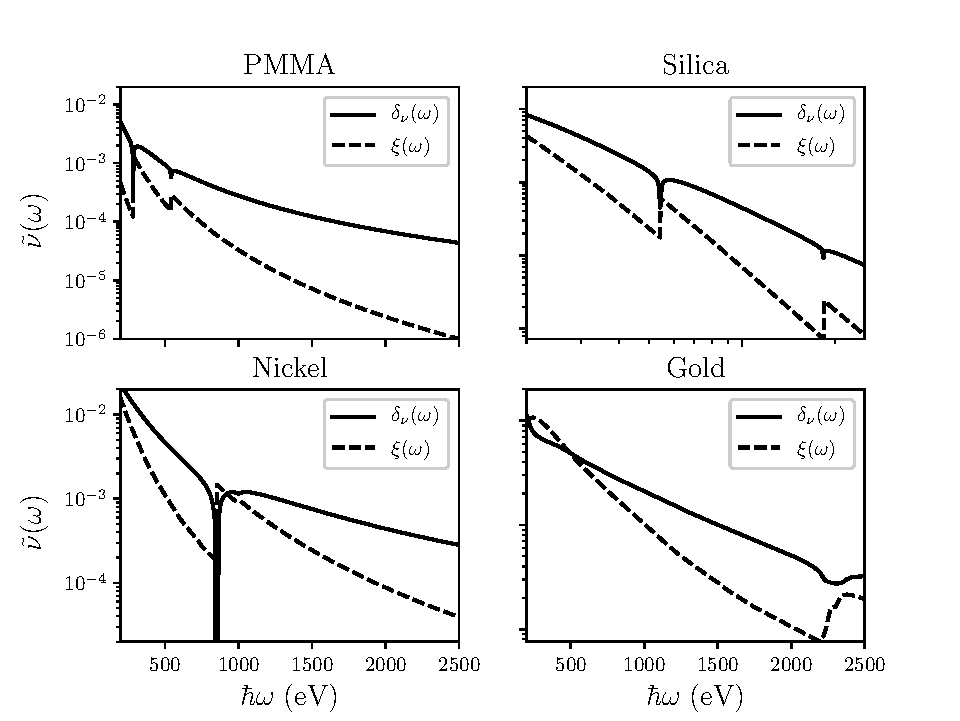
\includegraphics[scale=0.95]{Appendix-C/Figures/X-ray_index.pdf}
 \caption[Soft x-ray index of refraction for PMMA, silica, nickel and gold]{Soft x-ray index of refraction for PMMA (\ce{C5H8O2})$_n$, silica (\ce{SiO2}), nickel (\ce{Ni}) and gold (\ce{Au}) on a logarithmic scale \cite{CXRO_database}}\label{fig:X-ray_index} 
 \end{figure} 
PMMA and silica, as materials with molecular composition, have optical constants that depend on an average of the atomic scattering factors for the constituent atoms and as a result, multiple absorption edges are evident in these plots. 
Using these optical constants, the wave number in the medium now can be written as 
\begin{subequations}
\begin{equation}
 \tilde{k} \equiv \tilde{\nu} (\omega) k_0 = \frac{\omega}{c_0} \left[ 1 - \delta_{\nu} (\omega) + i \xi(\omega) \right] . 
 \end{equation}
For the special case of a wave decaying in the direction of propagation with $\mathbold{\tilde{k}} \cdot \mathbold{r} = \tilde{k} r$, the electric field is of the form
\begin{equation}
 \mathbold{E} \left( \mathbold{r} , t \right) = \mathbold{E}_0 \mathrm{e}^{i (\tilde{k} r - \omega t)} = \mathbold{E}_0 \mathrm{e}^{i k_0 \left( r - c_0 t \right)} \mathrm{e}^{i k_0 r \delta_{\nu} (\omega)} \mathrm{e}^{-k_0 r \xi(\omega)} ,
 \end{equation}
which indicates the medium induces a phase shift $k_0 r \delta_{\nu} (\omega)$ and causes the wave to decay exponentially with wave intensity dropping off as $\mathrm{e}^{- 2 k_0 r \xi(\omega)}$. 
The scattered wave therefore becomes \SI{1}{\radian} out of phase with the original wave over a distance known as the \emph{extinction length} \cite{deBergevin09}:
\begin{equation}\label{eq:extinction_length}
 k_0 r \delta_{\nu} (\omega) = 1 \implies \ell_{\text{ext}} \equiv \frac{\lambda}{2 \pi \delta_{\nu} (\omega)} ,
 \end{equation}
while on the other hand, the $1/\mathrm{e}$ length scale for absorption is \cite{Attwood17}:
\begin{equation}\label{eq:eabsorption_length}
 2 k_0 r \xi(\omega) = 1 \implies \ell_{\text{abs}} \equiv \frac{\lambda}{4 \pi \xi(\omega)} .
 \end{equation}
\end{subequations}
These two characteristic length scales are plotted in \cref{fig:X-ray_lengths} using the optical constants from \cref{fig:X-ray_index}. 
\begin{figure}
 \centering
 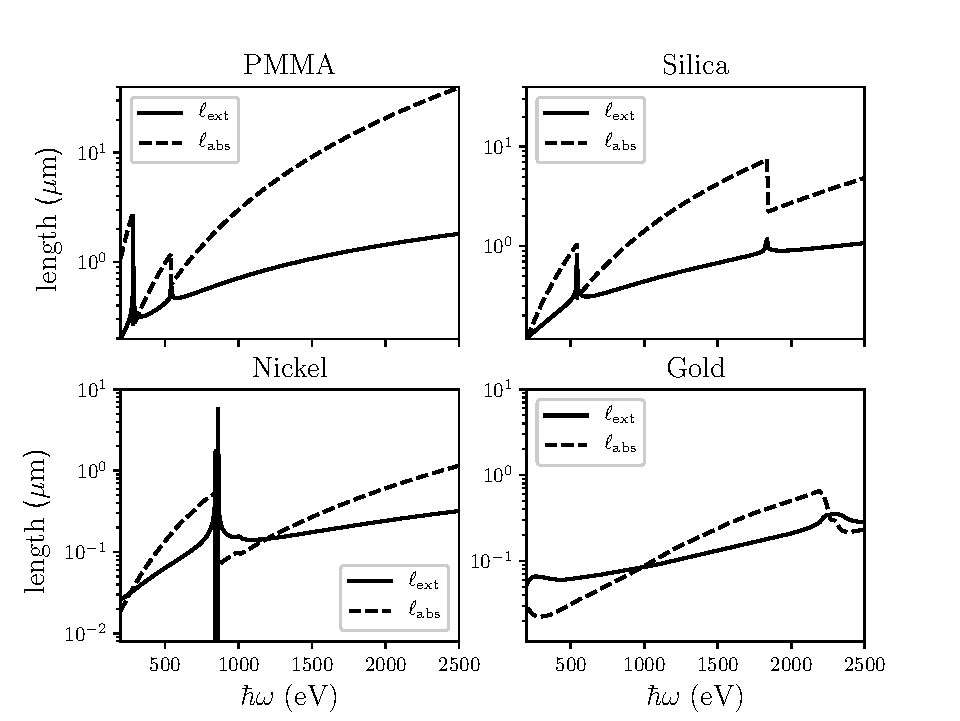
\includegraphics[scale=0.95]{Appendix-C/Figures/X-ray_lengths.pdf}
 \caption[Characteristic length scales for soft x-rays in PMMA, silica, nickel and gold]{Characteristic length scales for soft x-rays in PMMA (\ce{C5H8O2})$_n$, silica (\ce{SiO2}), nickel (\ce{Ni}) and gold (\ce{Au}). The extinction length, $\ell_{\text{ext}}$, arises from a phase shift due to the real index while $\ell_{\text{abs}}$ describes the length scale of absorption due to the imaginary index \cite{CXRO_database}}\label{fig:X-ray_lengths} 
 \end{figure} 
This demonstrates that soft x-rays are attenuated over short, sub-\si{\um} distances that decrease as $\mathcal{Z}$ increases, especially near prominent absorption edges. 

\section{Reflection from a Mirror Flat}\label{sec:planar_interface}
%%%%%%%%%%%%%%%%%%%%%%%%%%%%%%%%%%%%%%%%%--------------------------------------------------
Several important properties of reflective overcoats for x-ray reflection gratings can be gleaned from considering how a single mode of soft x-rays with frequency $\omega$ reflects and refracts at a planar interface between vacuum, with index of refraction equal to unity (\emph{i.e.}, $\tilde{\nu} (\omega) = \nu (\omega) = 1$) and a material that represents a thick mirror with a complex index of refraction, $\tilde{\nu} (\omega) \equiv \nu (\omega) + i \xi(\omega)$, where $\nu (\omega) \equiv 1 - \delta_{\nu} (\omega) \lessapprox 1$ and $\xi(\omega) \ll 1$ [\emph{cf.\@} \cref{sec:x-ray_index}]. 
To draw an analogy with radiation illuminating an idealized sawtooth facet of an x-ray reflection grating [\emph{cf.\@} \cref{fig:conical_reflection_edit}], the angle of incidence measured relative to the surface of the mirror is taken to be $\zeta$. 
Using the coordinate system defined in \cref{fig:2Dmirror_angles}, the incident wave vector given by 
\begin{subequations}
\begin{equation}\label{eq:2D_incident_wave}
 \mathbold{k} = k_x \mathbold{\hat{x}} + k_y \mathbold{\hat{y}} = k_0 \left[ \cos \left( \zeta \right) \mathbold{\hat{x}} - \sin \left( \zeta \right) \mathbold{\hat{y}} \right] 
 \end{equation}
with $\abs{\mathbold{k}} = k_0 \equiv 2 \pi / \lambda = \sqrt{k_x^2 + k_y^2}$ and $k_z = 0$. 
\begin{figure}
 \centering
 \includegraphics[scale=1.25]{Appendix-C/Figures/diffraction_arc22.mps}
 \caption[Geometry for in-plane reflection and refraction]{Geometry for in-plane reflection and refraction, where $\mathbold{k}$ is the incident wave vector, $\mathbold{k}''$ is the reflected wave vector and $\mathbold{\tilde{k}}'$ is the refracted wave vector.}\label{fig:2Dmirror_angles}
 \end{figure}
The corresponding electromagnetic wavefront is represented by 
\begin{equation} \label{eq:incident_fields}
 \mathbold{E} \left( x, y, z \right) = \mathbold{E}_0 \mathrm{e}^{i \left( k_x x + k_y y \right)} \text{ and } \mathbold{H} \left( x, y, z \right) = \frac{1}{Z_0 k_0} \mathbold{k} \times \mathbold{E} \left( x, y, z \right) ,
 \end{equation}
where $\mathbold{E}_0$ is a vector describing the polarization and amplitude of the incident electric field [\emph{cf.\@} \cref{sec:EM_waves_vac}]. 
\end{subequations}
Kept in arbitrary form, the reflected ray is also associated with a real wave vector: 
\begin{subequations}
\begin{equation}\label{eq:3D_reflected_wave_vector}
 \mathbold{k''} = k_x'' \mathbold{\hat{x}} + k_y'' \mathbold{\hat{y}} + k_z'' \mathbold{\hat{z}}
 \end{equation}
with $\abs{\mathbold{k''}} = k_0 = \sqrt{k_x^2 + k_y^2 + k_z^2}$ while the reflected wavefront can be written using 
\begin{equation}\label{eq:reflected_fields}
\mathbold{E''} \left( x, y, z \right) = \mathbold{E}_0'' \mathrm{e}^{i \left( k_x'' x + k_y'' y + k_z'' z \right)} \text{ and } \mathbold{H''} \left( x, y, z \right) = \frac{1}{Z_0 k_0} \mathbold{k''} \times \mathbold{E''} \left( x, y, z \right) ,
 \end{equation} 
where $\mathbold{E}_0''$ describes the polarization and amplitude of the reflected electric field.  
\end{subequations}
On the other hand, the refracted ray is described with a complex wave vector [\emph{cf.\@} \cref{eq:k_tilde_def}]:
\begin{subequations}
\begin{equation}\label{eq:3D_refracted_wave_vector}
 \mathbold{\tilde{k}'} = \mathbold{k'} + i \mathbold{\kappa'} = \tilde{k}_x' \mathbold{\hat{x}} + \tilde{k}_y' \mathbold{\hat{y}} + \tilde{k}_z' \mathbold{\hat{z}}
 \end{equation}
with $\abs{\mathbold{\tilde{k}'}} = \tilde{k}' \equiv \tilde{\nu} (\omega) \, k_0 = \sqrt{\tilde{k}_x'^2 + \tilde{k}_y'^2 + \tilde{k}_z'^2}$ and the refracted wavefront is associated with complex electromagnetic fields, where $\mathbold{E}_0'$ describes the polarization and initial amplitude of the refracted electric field: 
\begin{equation}\label{eq:refracted_fields}
 \mathbold{E'} \left( x, y, z \right) = \mathbold{E}_0' \mathrm{e}^{i \left( \tilde{k_x}' x + \tilde{k_y}' y + \tilde{k_z}' z \right)} \text{ and } \mathbold{H'} \left( x, y, z \right) = \frac{1}{Z_0 k_0} \mathbold{\tilde{k}'} \times \mathbold{E'} \left( x, y, z \right) .
 \end{equation} 
\end{subequations}

To describe rigorously how the reflected and refracted fields are related to the incident wave, the Helmholtz equation [\emph{cf.\@} \cref{eq:Helmholtz}] is solved above the mirror surface, in vacuum:
\begin{subequations}
\begin{equation} 
 \left( \laplacian + k_0^2 \right) \left\{
 \begin{array}{lr}
 \mathbold{E} \left( x, y, z \right) + \mathbold{E''} \left( x, y, z \right) \\
 \mathbold{H} \left( x, y, z \right) + \mathbold{H''} \left( x, y, z \right) \label{eq:Helmholtz_above_mirror}
 \end{array}
 \right\} = \mathbf{0} ,
 \end{equation}
and below the surface, in a dispersive medium representing the mirror material [\emph{cf.\@} \cref{eq:Helmholtz_med}]:
\begin{equation} 
 \left( \laplacian + \tilde{k}'^2 \right) \left\{
 \begin{array}{lr}
 \mathbold{E'} \left( x, y, z \right) \\
 \mathbold{H'} \left( x, y, z \right) \label{eq:Helmholtz_below_mirror}
 \end{array}
 \right\} = \mathbf{0} . 
 \end{equation}
\end{subequations}
Additionally, the incident, reflected and refracted fields must be phase-matched across the boundary, which is initially taken to be a perfectly smooth plane representing the surface of the mirror at $y=0$. 
This can be handled using the general boundary conditions for electrodynamics in the absence of surface current and surface charge \cite{Landau60,Jackson75}: 
\begin{subequations}
\begin{align}
 \mathbold{\hat{n}} \times \left[ \mathbold{E} \left( x, 0, z \right) + \mathbold{E''} \left( x, 0, z \right) \right] &= \mathbold{\hat{n}} \times \mathbold{E'} \left( x, 0, z \right) \label{eq:general_boundary_1} \\
 \mathbold{\hat{n}} \times \left[\mathbold{H} \left( x, 0, z \right)  + \mathbold{H''} \left( x, 0, z \right) \right] &= \mathbold{\hat{n}} \times \mathbold{H'} \left( x, 0, z \right) \label{eq:general_boundary_2} \\
 \mathbold{\hat{n}} \cdot \left[ \mathbold{E} \left( x, 0, z \right) + \mathbold{E''} \left( x, 0, z \right) \right] &= \tilde{\nu}^2 (\omega) \, \mathbold{\hat{n}} \cdot \mathbold{E'} \left( x, 0, z \right) \label{eq:general_boundary_3} \\
 \mathbold{\hat{n}} \cdot \left[ \mathbold{H} \left( x, 0, z \right) + \mathbold{H''} \left( x, 0, z \right) \right] &= \mathbold{\hat{n}} \cdot \mathbold{H'} \left( x, 0, z \right) \label{eq:general_boundary_4} , 
 \end{align}
\end{subequations}
where $\mathbold{\hat{n}} = \mathbold{\hat{y}}$ is a unit vector pointing from the dispersive medium to vacuum [\emph{cf.\@} \cref{fig:2Dmirror_angles}]. 
Inserting \cref{eq:incident_fields,eq:reflected_fields,eq:refracted_fields} into these relations verifies that reflection and refraction occur in-plane with the requirement that $k_z \equiv 0 = k_z'' = \tilde{k_z}'$. 
These boundary conditions also demand that $k_x = k_x'' = \tilde{k_x}'$, which leads to the \emph{law of reflection} and \emph{Snell's law of refraction}. 
Explicitly, with $k_x'' \equiv k_0 \cos \left( \zeta '' \right)$ the former reads as 
\begin{equation}\label{eq:reflection}
 k_x'' = k_x \implies \zeta'' = \zeta ,
 \end{equation}
where $k_y'' \equiv k_0 \sin \left( \zeta '' \right)$. 
Meanwhile, $\tilde{k_x}' \equiv \tilde{k}' \cos \left( \tilde{\zeta}' \right)$ is associated with a complex angle, $\tilde{\zeta}'$, so that the latter reads as
%\begin{subequations}
\begin{subequations}
\begin{equation}\label{eq:refraction}
  \tilde{k_x}' = k_x \implies \tilde{\nu}(\omega) \cos \left( \tilde{\zeta}' \right) = \cos \left( \zeta \right) 
 \end{equation}
with $\tilde{k_y}' \equiv - \tilde{k}' \sin \left( \tilde{\zeta}' \right)$. 
Defining $\tilde{\zeta}' \equiv \zeta'_{\Re} + i \zeta'_{\Im}$ and using a trigonometric identity involving complex angles,\footnote{$\cos \left( \zeta'_{\Re} + i \zeta'_{\Im}\right) = \cos \left( \zeta'_{\Re} \right) \cosh \left( \zeta'_{\Im} \right) - i \sin \left( \zeta'_{\Re} \right) \sinh \left( \zeta'_{\Im} \right)$} \cref{eq:refraction} yields the following relations:
\begin{align}
 \nu (\omega) \cos \left( \zeta'_{\Re} \right) \cosh \left( \zeta'_{\Im} \right) + \xi (\omega) \sin \left( \zeta'_{\Re} \right) \sinh \left( \zeta'_{\Im} \right) &= \cos \left( \zeta \right) \label{eq:refractionA} \\
 \xi (\omega) \cos \left( \zeta'_{\Re} \right) \cosh \left( \zeta'_{\Im} \right) - \nu (\omega) \sin \left( \zeta'_{\Re} \right) \sinh \left( \zeta'_{\Im} \right) &=0 \label{eq:refractionB} ,
 \end{align}
\end{subequations}
which imply that $\zeta'_{\Im} = 0$ if $\xi (\omega) = 0$. 

Crucially, appreciable reflectivity from an interface at soft x-ray frequencies can only be achieved in the regime of \emph{total external reflection (TER)}, where $\zeta$ is small enough such that the refracted ray travels virtually parallel to the surface of the mirror with $\zeta'_{\Re} \approx 0$ instead of propagating down into the dispersive medium substantially. 
\begin{figure}
 \centering
 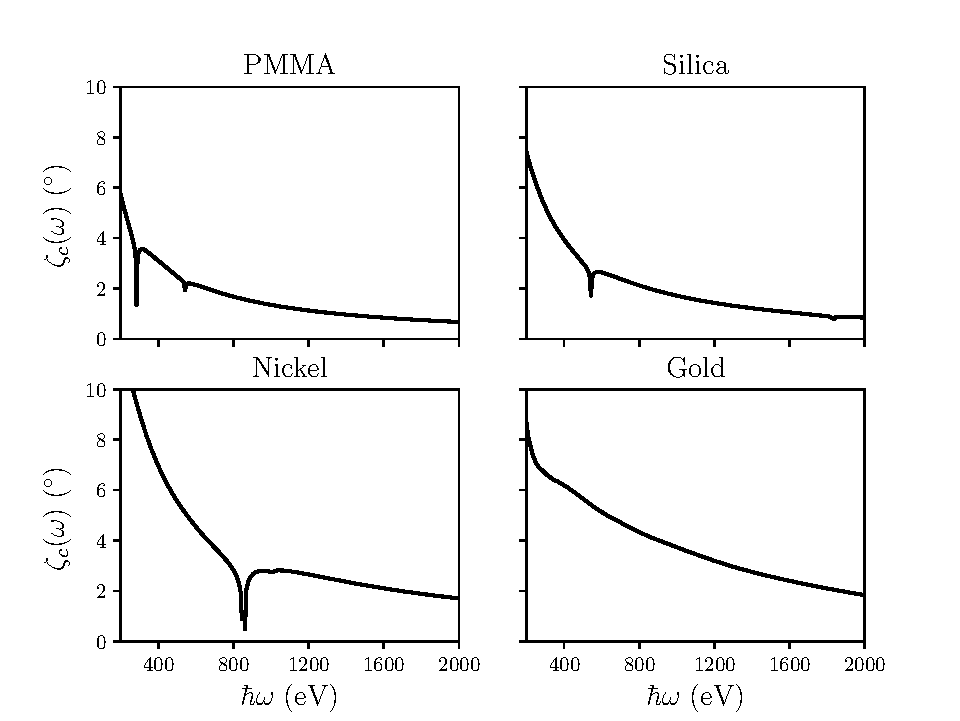
\includegraphics[scale=0.95]{Appendix-C/Figures/critical_angle.pdf}
 \caption[Critical angle for total external reflection (TER) of PMMA, silica, nickel and gold across the soft x-ray spectrum]{Critical angle for total external reflection (TER) of PMMA (\ce{C5H8O2})$_n$, silica (\ce{SiO2}), nickel (\ce{Ni}) and gold (\ce{Au}) across the soft x-ray spectrum \cite{CXRO_database}}\label{fig:critical_angle}
 \end{figure} 
While this is shown explicitly in \cref{sec:reflectivity_polarization,sec:total_refl}, it can be gleaned by neglecting $\xi (\omega)$ for the moment so that $\tilde{\nu} (\omega) = \nu (\omega) \lessapprox 1$ and $\zeta'_{\Im} = 0$ with \cref{eq:refractionA} reducing to 
\begin{equation}\label{eq:Snell_real}
 \cos \left( \zeta \right) = \nu (\omega) \cos \left( \zeta'_{\Re} \right) . 
 \end{equation}
From this expression, the condition for TER is met when $\zeta$ is smaller than a certain \emph{critical angle}, $\zeta_c (\omega)$, that corresponds to $\zeta'_{\Re} = 0$ with $\cos \left( \zeta \right) = \nu (\omega) \equiv 1 - \delta_{\nu} (\omega)$. 
This can be written as
\begin{equation}\label{eq:critical_angle}
 \zeta_c (\omega) \equiv \arccos \left[ 1 - \delta_{\nu} (\omega) \right] \approx \sqrt{2 \delta_{\nu} (\omega)} ,
 \end{equation}
where the approximation is valid for $\delta_{\nu} (\omega) \ll 1$ \cite{Attwood17}. 
Using data for $\delta_{\nu} (\omega)$ obtained from CXRO \cite{CXRO_database}, $\zeta_c (\omega)$ is plotted as a function of photon energy in \cref{fig:critical_angle} for the materials from \cref{fig:X-ray_index,fig:X-ray_lengths}, where it is seen that $\zeta \lessapprox 2^{\circ}$ is typically required to achieve TER across the soft x-ray bandpass. 

The term \emph{total external reflection} by name implies that all incident radiation is reflected from a mirror with $\nu (\omega) < 1$. 
Although this is approximately true, a real material with a complex index of refraction, $\tilde{\nu} (\omega)$, has an imaginary part, $\xi(\omega) \neq 0$, that takes into account losses in reflectivity and additionally, causes the refracted ray to penetrate slightly into the mirror rather than travel parallel to the surface as deduced above \cite{Attwood17}. 
The former is quantified by analyzing the \emph{Fresnel equations} for specular reflectivity in \cref{sec:reflectivity_polarization} while the latter [\emph{cf.\@} \cref{sec:total_refl}] manifests as a \emph{penetration depth} that informs thickness requirements for reflective overcoats. 
Moreover, the presence of surface roughness leads to losses in specular reflectivity in a manner that depends on the size scale of surface features and the wave vector of incident radiation [\emph{cf.\@} \cref{sec:rough_surface}]. % this is the subject of \cref{sec:rough_surface}. 

\subsection{Fresnel Reflectivity in Orthogonal Polarizations}\label{sec:reflectivity_polarization}
%%%%%%%%%%%%%%%%%%%%%%%%%%%%%%%%%%%%%%%%%--------------------------------------------------
The reflectivity of a mirror flat that can be regarded as being infinitely thick\footnote{In practice, this means that a slab of material is assumed to be thick enough for the refracted ray to be completely absorbed before reaching another interface.} is defined as the ratio of the specularly-reflected and incident waves in terms of flux through a unit area of a surface parallel to the boundary \cite{Born80}. 
Using $\mathbold{S}(\mathbold{r}) = \mathbold{E}(\mathbold{r}) \times \mathbold{H}(\mathbold{r})$ as the time-harmonic form of \emph{Poynting's vector} \cite{Griffiths17,Jackson75}, this can be written as 
\begin{equation}\label{eq:fresnel_refl_def}
 \mathcal{R}_F \equiv \frac{\mathbold{S}''(\mathbold{r}) \cdot \mathbold{\hat{y}}}{\mathbold{S}(\mathbold{r}) \cdot \mathbold{\hat{y}}} = \frac{k_y''}{k_y} \frac{\abs{\mathbold{E}_0''}^2}{\abs{\mathbold{E}_0}^2} = \frac{\abs{\mathbold{E}_0''}^2}{\abs{\mathbold{E}_0}^2} ,
 \end{equation} 
which reduces to ratio of field strengths for the incident and reflected waves. 
By symmetry, the boundary conditions [\emph{cf.\@} \cref{eq:general_boundary_1,eq:general_boundary_2,eq:general_boundary_3,eq:general_boundary_4}] demand that the time-harmonic electromagnetic fields are constant across the surface of the mirror, except for a phase shift that depends on the parallel component of the wave number, $k_{\parallel}$. 
Using the coordinate system defined in \cref{fig:2Dmirror_angles}, where $k_z = 0$ by construction, $k_{\parallel} \equiv k_x = k_0 \cos \left( \zeta \right)$ so that translations in $x$ on the boundary come with a $\mathrm{e}^{i k_x x}$ dependence while translations in $z$ introduce no phase shift. 
This allows the electromagnetic fields at the surface of the mirror to be described as being \emph{space-harmonic} such that the time-harmonic incident fields can be written as
\begin{equation}
 \left\{
 \begin{array}{lr}
 \mathbold{E} \left( \mathbold{r} \right) \\
 \mathbold{H} \left( \mathbold{r} \right)
 \end{array} 
 \right\} =  \left\{
 \begin{array}{lr}
 \mathbold{E} \left( y \right) \\
 \mathbold{H} \left( y \right)
 \end{array} 
 \right\} \mathrm{e}^{i k_x x} \underbrace{\mathrm{e}^{i k_z z}}_1 
 \end{equation} 
with similar expressions for the reflected and refracted fields. 
The Helmholtz equations given by \cref{eq:Helmholtz_above_mirror,eq:Helmholtz_below_mirror} then reduce to 
\begin{subequations}
\begin{equation} 
 \left( \frac{d^2}{d y^2} + k_y^2 \right) \left\{
 \begin{array}{lr}
 \mathbold{E} \left( y \right) + \mathbold{E''} \left( y \right) \\
 \mathbold{H} \left( y \right) + \mathbold{H''} \left( y \right) \label{eq:Helmholtz_above_mirror_simplified}
 \end{array}
 \right\} = \mathbf{0} 
 \end{equation}
in vacuum with $k_y^2 = k_0^2 - k_x^2 = k_0^2 \sin^2 \left( \zeta \right)$ and 
\begin{equation} 
 \left( \frac{d^2}{d y^2} + \tilde{k_y}'^2 \right) \left\{
 \begin{array}{lr}
 \mathbold{E'} \left( y \right) \\
 \mathbold{H'} \left( y\right) \label{eq:Helmholtz_below_mirror_simplified}
 \end{array}
 \right\} = \mathbf{0} 
 \end{equation}
inside the material of the mirror with $\tilde{k_y}'^2 = \tilde{k}'^2 - k_x^2 = k_0^2 \left[ \tilde{\nu}^2(\omega) - \cos^2 \left( \zeta \right) \right]$. 
\end{subequations}

The incident wave is assumed to be traveling toward the mirror surface with a $\mathrm{e}^{i k_y y}$ dependence, where $k_y \equiv -k_0 \sin \left( \zeta \right)$ [\emph{cf.\@} \cref{eq:2D_incident_wave,fig:2Dmirror_angles}]. 
Meanwhile, the reflected wave travels away with a $\mathrm{e}^{-i k_y y}$ dependence so that the total electric field in vacuum can be written as 
\begin{subequations}
\begin{equation}
 \mathbold{E} \left( y \right) + \mathbold{E''} \left( y \right) = \mathbold{E}_0 \mathrm{e}^{i k_y y} + \mathbold{E}_0'' \mathrm{e}^{-i k_y y} ,
 \end{equation}
which is a solution to \cref{eq:Helmholtz_above_mirror}. 
On the other hand, a physically-realistic solution to \cref{eq:Helmholtz_below_mirror_simplified} is one which propagates away from the surface, into the mirror with
\begin{equation}
 \mathbold{E'} \left( y \right) = \mathbold{E}_0' \mathrm{e}^{i \tilde{k_y}' y} 
 \end{equation}
\end{subequations}
so that using \cref{eq:incident_fields,eq:reflected_fields,eq:refracted_fields} for the corresponding magnetic fields, the boundary conditions given by \cref{eq:general_boundary_1,eq:general_boundary_2,eq:general_boundary_3,eq:general_boundary_4} reduce to
\begin{subequations}
\begin{align} 
 \mathbold{\hat{y}} \times \left[ \mathbold{E}_0 + \mathbold{E}_0'' \right] &= \mathbold{\hat{y}} \times \mathbold{E}_0' \label{eq:mirror_boundary_1} \\
 \mathbold{\hat{y}} \times \left[ \mathbold{k} \times \mathbold{E}_0 + \mathbold{k''} \times \mathbold{E}_0'' \right] &= \mathbold{\hat{y}} \times \left[ \mathbold{\tilde{k}'} \times \mathbold{E}_0' \right] \label{eq:mirror_boundary_2} \\
 \mathbold{\hat{y}} \cdot \left[ \mathbold{E}_0 + \mathbold{E}_0'' \right] &= \tilde{\nu}^2 (\omega) \, \mathbold{\hat{y}} \cdot \mathbold{E}_0' \label{eq:mirror_boundary_3} \\
 \mathbold{\hat{y}} \cdot \left[ \mathbold{k} \times \mathbold{E}_0 + \mathbold{k''} \times \mathbold{E}_0'' \right] &= \mathbold{\hat{y}} \cdot \left[ \mathbold{\tilde{k}'} \times \mathbold{E}_0' \right] \label{eq:mirror_boundary_4} .
 \end{align} %This shows that polarization is the same for incident, refracted and reflected rays?
\end{subequations}
To evaluate how polarization, given by the orientation of the electric field vector, affects the reflectivity of a mirror, the Helmholtz equations given by \cref{eq:Helmholtz_above_mirror_simplified,eq:Helmholtz_below_mirror_simplified} are solved with the boundary conditions defined in \cref{eq:mirror_boundary_1,eq:mirror_boundary_2,eq:mirror_boundary_3,eq:mirror_boundary_4}, in two orthogonal, linear polarization states:
\begin{itemize}[noitemsep]
  \item \emph{s-polarization}: the electric field is perpendicular to the plane of incidence and parallel to the surface, and 
  \item \emph{p-polarization}: the electric field is parallel to the plane of incidence and perpendicular to the the surface, 
\end{itemize}
with $u(y)$ as a scalar function representing the magnitude of the field in each case. 
Similarly, from \cref{eq:mirror_boundary_1,eq:mirror_boundary_2,eq:mirror_boundary_3,eq:mirror_boundary_4}, the reflected and refracted fields can also be represented with scalar functions $u''(y)$ and $u'(y)$, respectively, and \cref{eq:Helmholtz_above_mirror_simplified,eq:Helmholtz_below_mirror_simplified} are reduced to their scalar form:
\begin{subequations}
\begin{align}
 \left( \dv[2]{y} + k_y^2 \right) \left[ u(y) + u''(y)  \right] &= 0 \quad \text{for $y>0$} \\
 \left( \dv[2]{y} + \tilde{k_y}'^2 \right) u'(y) &= 0 \quad \text{for $y<0$} .
  \end{align}
 \end{subequations}
Solving these equations for each orthogonal polarization allows the reflectivity in any arbitrary polarization to determined through superposition. 

The incident, reflected and refracted electric fields in s-polarization, which are parallel to the surface of the mirror, can be written as
\begin{align}
\begin{split}
 \mathbold{E}(y) &= \mathcal{A}_s \mathbold{\hat{z}} \mathrm{e}^{i k_y y} \quad \text{(incident)} \quad \quad \mathbold{E''}(y) = \mathcal{A}_s'' \mathbold{\hat{z}} \mathrm{e}^{-i k_y y} \quad \text{(reflected)} \\
 \mathbold{E'}(y) &= \mathcal{A}_s' \mathbold{\hat{z}} \mathrm{e}^{i \tilde{k_y}' y} \quad \text{(refracted/attenuated)} ,
 \end{split}
 \end{align}
where $\mathcal{A}_s$ is the known amplitude of the incident electric field while $\mathcal{A}_s''$ and $\mathcal{A}_s'$ are the unknown amplitudes of the reflected and refracted electric fields. 
From \cref{eq:mirror_boundary_1,eq:mirror_boundary_2,eq:mirror_boundary_3,eq:mirror_boundary_4}, the boundary conditions for this polarization give\footnote{Here, the following vector triple product rules have been used: $\mathbold{A} \times \left( \mathbold{B} \times \mathbold{C} \right) = \left( \mathbold{A} \cdot \mathbold{C} \right) \mathbold{B} - \left( \mathbold{A} \cdot \mathbold{B} \right) \mathbold{C}$ and $\mathbold{A} \cdot \left( \mathbold{B} \times \mathbold{C} \right) = \mathbold{B} \cdot \left( \mathbold{C} \times \mathbold{A} \right) = \mathbold{C} \cdot \left( \mathbold{A} \times \mathbold{B} \right)$.}  
\begin{subequations}
\begin{align}
%\begin{split}
 \mathbold{\hat{y}} \times \left[ \mathcal{A}_s \mathbold{\hat{z}} + \mathcal{A}_s'' \mathbold{\hat{z}} \right] = \mathbold{\hat{y}} \times \mathcal{A}_s' \mathbold{\hat{z}} &\implies \mathcal{A}_s + \mathcal{A}_s'' = \mathcal{A}_s' \\
 \mathbold{\hat{y}} \times \left[ \mathbold{k} \times \mathcal{A}_s \mathbold{\hat{z}}  + \mathbold{k''} \times \mathcal{A}_s'' \mathbold{\hat{z}} \right] = \mathbold{\hat{y}} \times \left[ \mathbold{\tilde{k}'} \times \mathcal{A}_s' \mathbold{\hat{z}} \right] &\implies \left( \mathcal{A}_s - \mathcal{A}_s'' \right) k_y = \mathcal{A}_s' \tilde{k_y}' \\ 
 \mathbold{\hat{y}} \cdot \left[ \mathcal{A}_s \mathbold{\hat{z}'} + \mathcal{A}_s'' \mathbold{\hat{z}'} \right] = \tilde{\nu}^2 (\omega) \, \mathbold{\hat{y}} \cdot \mathcal{A}_s' \mathbold{\hat{z}'} &\implies 0 = 0 \\
 \mathbold{\hat{y}} \cdot \left[ \mathbold{k} \times \mathcal{A}_s \mathbold{\hat{z}} + \mathbold{k''} \times \mathcal{A}_s'' \mathbold{\hat{z}} \right] = \mathbold{\hat{y}} \cdot \left[ \mathbold{\tilde{k}'} \times \mathcal{A}_s' \mathbold{\hat{z}} \right] &\implies \mathcal{A}_s + \mathcal{A}_s'' = \mathcal{A}_s' ,
 %\end{split}
 \end{align}
\end{subequations}
which can be rearranged to yield complex coefficients for reflection and transmission, respectively:
\begin{equation}\label{eq:s_coeff}
 \tilde{r}_s \equiv \frac{\mathcal{A}_s''}{\mathcal{A}_s} = \frac{k_y - \tilde{k_y}'}{k_y + \tilde{k_y}'} \quad \text{and} \quad \tilde{t}_s \equiv \frac{\mathcal{A}_s'}{\mathcal{A}_s} = \frac{2 k_y}{k_y + \tilde{k_y}'} 
 \end{equation}
with $k_y = - k_0 \sin (\zeta)$ and $\tilde{k_y}' = - \sqrt{\tilde{\nu}^2 (\omega) - \cos^2 \left( \zeta \right)}$. 
While the \emph{transmissivity} of a mirror in s-polarization depends on $\tilde{t}_s$, the reflectivity is determined from
\begin{equation}\label{eq:s_reflectivity}
 \mathcal{R}_s (\zeta) = \norm{\tilde{r}_s}^2 = \norm{\left( \frac{\sin \left( \zeta \right) - \sqrt{\tilde{\nu}^2 (\omega) - \cos^2 \left( \zeta \right)}}{\sin \left( \zeta \right) + \sqrt{\tilde{\nu}^2 (\omega) - \cos^2 \left( \zeta \right)}} \right)}^2 .
 \end{equation}
In p-polarization on the other hand, the incident, reflected and refracted electric fields are perpendicular to the surface of the mirror. 
The corresponding magnetic fields are then parallel to the surface, which can be written as 
\begin{subequations}
\begin{align}
\begin{split}
 \mathbold{H} (y) &= \frac{\mathcal{A}_p}{Z_0} \mathbold{\hat{z}} \mathrm{e}^{i k_y y} \quad \text{(incident)} \quad \quad \mathbold{H''} (y) = \frac{\mathcal{A''}_p}{Z_0} \mathbold{\hat{z}} \mathrm{e}^{-i k_y y} \quad \text{(reflected)} \\
 \mathbold{H'} (y) &= \frac{\mathcal{A'}_p}{Z_0} \mathbold{\hat{z}} \mathrm{e}^{i \tilde{k_y}' y} \quad \text{(refracted/attenuated)} ,
 \end{split}
 \end{align} 
\end{subequations}
where $\mathcal{A}_p$ is the known amplitude of the incident electric field, while $\mathcal{A}_p''$ and $\mathcal{A}_p'$ are the unknown amplitudes of the reflected and refracted electric fields. 
Using \cref{eq:Maxwell_vac_FT_4,eq:Maxwell_med_FT_4} for the electric field, the boundary conditions for this polarization yield 
\begin{subequations}
\begin{align}
%\begin{split}
 \mathbold{\hat{y}} \times \left[\mathbold{k} \times \mathcal{A}_p \mathbold{\hat{z}} + \mathbold{k''} \times \mathcal{A}_p'' \mathbold{\hat{z}} \right] = \mathbold{\hat{y}} \times \left[ \frac{\mathbold{\tilde{k}'}  \times \mathcal{A}_p' \mathbold{\hat{z}}}{\tilde{\nu}^2(\omega)} \right] &\implies \left( \mathcal{A}_p - \mathcal{A}_p'' \right) k_y = \frac{\mathcal{A}_p' \tilde{k_y}'}{\tilde{\nu}^2(\omega)} \\ 
 \mathbold{\hat{y}} \times \left[ \mathcal{A}_p \mathbold{\hat{z}} + \mathcal{A}_p'' \mathbold{\hat{z}} \right] = \mathbold{\hat{y}} \times \mathcal{A}_p' \mathbold{\hat{z}} &\implies \mathcal{A}_p + \mathcal{A}_p'' = \mathcal{A}_p' \\
 \mathbold{\hat{y}} \cdot \left[ \mathbold{k} \times \mathcal{A}_p \mathbold{\hat{z}} + \mathbold{k''} \times \mathcal{A}_p'' \mathbold{\hat{z}} \right] = \mathbold{\hat{y}} \cdot \left[\mathbold{\tilde{k}'}  \times \mathcal{A}_p' \mathbold{\hat{z}} \right] &\implies \mathcal{A}_p + \mathcal{A}_p'' = \mathcal{A}_p' \\
 \mathbold{\hat{y}} \cdot \left[ \mathcal{A}_p \mathbold{\hat{z}} + \mathcal{A}_p'' \mathbold{\hat{z}} \right] = \mathbold{\hat{y}} \cdot \mathcal{A}_p' \mathbold{\hat{z}} &\implies 0 = 0 .
 %\end{split}
 \end{align}
\end{subequations}
These expressions can be rearranged as
\begin{equation}\label{eq:p_coeff}
 \tilde{r}_p \equiv \frac{\mathcal{A}_p''}{\mathcal{A}_p} = \frac{\tilde{\nu}^2(\omega) k_y  - \tilde{k_y}'}{\tilde{k_y}' + \tilde{\nu}^2(\omega) k_y} \quad \text{and} \quad \tilde{t}_p \equiv \frac{\mathcal{A}_p'}{\mathcal{A}_p} = \frac{2 \tilde{\nu}^2(\omega) k_y}{\tilde{k_y}' + \tilde{\nu}^2(\omega) k_y} , 
 \end{equation}
with the former giving the following expression for reflectivity in p-polarization:
\begin{equation}\label{eq:p_reflectivity}
 \mathcal{R}_p (\zeta) = \norm{\tilde{r}_p}^2 = \norm{\left( \frac{\tilde{\nu}^2 (\omega) \sin \left( \zeta \right) - \sqrt{\tilde{\nu}^2 (\omega) - \cos^2 \left( \zeta \right)}}{\tilde{\nu}^2 (\omega) \sin \left( \zeta \right) + \sqrt{\tilde{\nu}^2 (\omega) - \cos^2 \left( \zeta \right)}} \right)}^2 .
 \end{equation}

The expressions for $\mathcal{R}_s$ and $\mathcal{R}_p$ in \cref{eq:s_reflectivity,eq:p_reflectivity} are the reflection coefficients found in the \emph{Fresnel equations} \cite{Landau60,Jackson75,Born80,Griffiths17,Attwood17,Fresnel1823}, which assume a perfectly smooth surface. 
However, these expressions can be simplified in the soft x-ray regime with $\nu (\omega) \lessapprox 1$ and $\xi(\omega) \ll 1$ using 
\begin{subequations}
\begin{equation}\label{eq:index_approx}
 \tilde{\nu}^2 (\omega) = \nu^2 (\omega) + 2 i \nu(\omega) \xi(\omega) - \xi^2(\omega) \approx \nu^2 (\omega) + 2 i \xi(\omega) ,
 \end{equation}
where $\nu^2 (\omega) = \left[ 1 - \zeta^2_c (\omega) / 2 \right]^2 \approx 1 - \zeta^2_c (\omega)$ from the approximate definition of $\zeta_c (\omega)$ given by \cref{eq:critical_angle} \cite{Attwood17}. 
Then, \cref{eq:index_approx} becomes
\begin{equation}
 \tilde{\nu}^2 (\omega) \approx 1 - \zeta^2_c (\omega) + 2 i \xi(\omega) ,
 \end{equation}
\end{subequations}
and additionally, at grazing-incidence angles with $\zeta \ll 1$ it is justified to use the approximations $\sin \left( \zeta \right) \approx \zeta$ and $\cos^2 \left( \zeta \right) \approx 1 - \zeta^2$ so that the reflection coefficients can be written as  
\begin{subequations}
\begin{equation}\label{eq:s_refl_approx}
 \tilde{r}_s \approx \left( \frac{\zeta - \sqrt{\zeta^2 - \zeta^2_c (\omega) + 2 i \xi(\omega)}}{\zeta + \sqrt{\zeta^2 - \zeta^2_c (\omega) + 2 i \xi(\omega)}} \right)\quad \text{and} 
 \end{equation}
\begin{equation}\label{eq:p_refl_approx}
 \tilde{r}_p \approx \left( \frac{\zeta \left[ 1 - \zeta^2_c (\omega) + 2 i \xi(\omega) \right] - \sqrt{\zeta^2 - \zeta^2_c (\omega) + 2 i \xi(\omega)}}{\zeta \left[ 1 - \zeta^2_c (\omega) + 2 i \xi(\omega) \right] + \sqrt{\zeta^2 - \zeta^2_c (\omega) + 2 i \xi(\omega)}} \right) . 
 \end{equation}
\end{subequations}
Knowing that $\xi(\omega) \, \zeta  \ll  1$ and $\zeta^2_c (\omega) \zeta  \ll  1$ with $\zeta  \ll  1$, these relations indicate that reflectivity in s- and p-polarizations are virtually equal to each other at grazing-incidence angles (\emph{i.e.}, $\mathcal{R}_F \approx \mathcal{R}_s \approx \mathcal{R}_p$). 
\begin{figure}
 \centering
 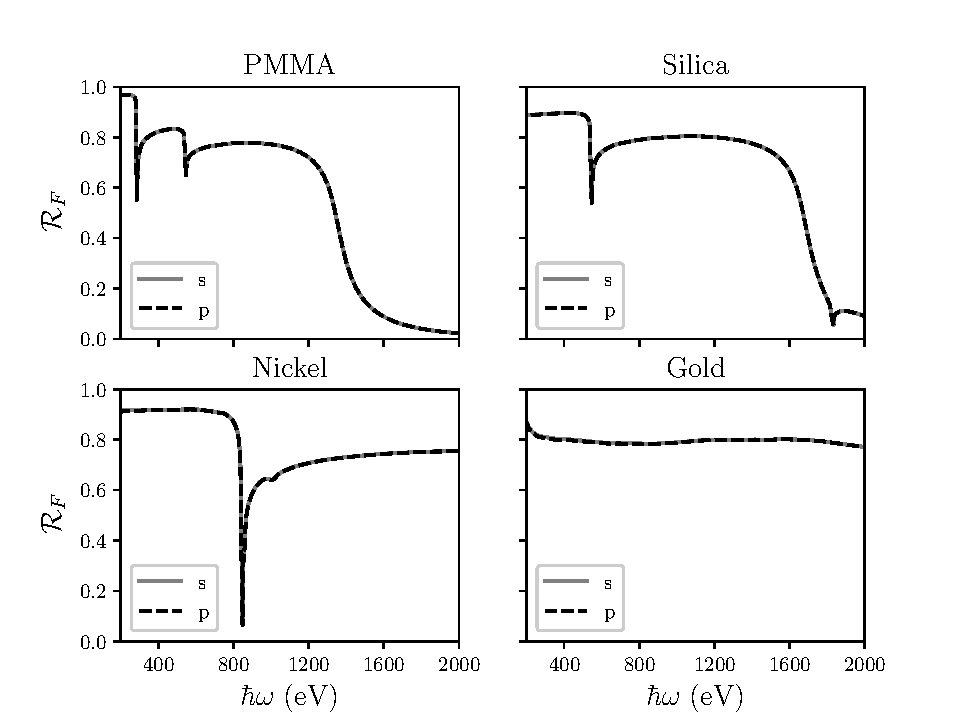
\includegraphics[scale=0.95]{Appendix-C/Figures/X-ray_refl.pdf}
 \caption[Fresnel soft x-ray reflectivity in orthogonal polarizations at a $1^{\circ}$ graze angle for PMMA, silica, nickel and gold]{Fresnel soft x-ray reflectivity in orthogonal polarizations at $\zeta = 1^{\circ}$ for PMMA (\ce{C5H8O2})$_n$, silica (\ce{SiO2}), nickel (\ce{Ni}) and gold (\ce{Au}), demonstrating lack of polarization sensitivity \cite{CXRO_database}}\label{fig:X-ray_refl}
 \end{figure} 
This is demonstrated graphically in \cref{fig:X-ray_refl}, where reflectivity data gathered from CXRO \cite{CXRO_database} are plotted for the materials from \cref{fig:X-ray_index,fig:X-ray_lengths,fig:critical_angle}.\footnote{Note, however, that the condition for TER, $\zeta = 1^{\circ} < \zeta_c (\omega)$, is not satisfied toward the blue end of the soft x-ray spectrum for PMMA and silica, which causes reflectivity to approach very small values.} 

With an insensitivity to polarization at grazing incidence, the expressions for $\mathcal{R}_s$ formulated above can be used to describe Fresnel reflectivity for a substrate or a thick slab of material (\emph{i.e.}, $\mathcal{R}_{\text{slab}} \equiv \mathcal{R}_F \approx \mathcal{R}_s$). 
For oxidizing materials, however, a thin film of oxide can form on a surface exposed to air. 
As alluded to in \cref{sec:crystal_etching}, this is the case for a silicon substrate with a layer of native oxide (\ce{SiO2}) that is a few \si{\nm} thick; another example is nickel oxide (NiO) forming on a layer of nickel. 
In any such case, taking $\tilde{\nu}_1 (\omega)$ as the complex index of refraction for the oxide layer, the complex reflection coefficient for the first interface in s-polarization is given by 
\begin{subequations}
\begin{equation}\label{eq:refl_coeff01}
 \tilde{r}_{0,1} = \frac{k_{y,0} - \tilde{k}_{y,1}}{k_{y,0} + \tilde{k}_{y,1}} = \frac{\sin \left( \zeta \right) - \sqrt{\tilde{\nu}_1^2 (\omega) - \cos^2 \left( \zeta \right)}}{\sin \left( \zeta \right) + \sqrt{\tilde{\nu}_1^2 (\omega) - \cos^2 \left( \zeta \right)}} ,
 \end{equation}
where $k_{y,0} = k_0 \sin \left( \zeta \right)$ and $\tilde{k}_{y,1} = k_0 \sqrt{\tilde{\nu}_1^2 (\omega) - \cos^2 \left( \zeta \right)}$ are the components of the wave vector normal to the boundary, in vacuum and in the oxide layer, respectively. 
Similarly, with $\tilde{\nu}_2 (\omega)$ as the complex index of refraction for the bulk material,\footnote{\emph{e.g.}, a silicon substrate or a relatively thick nickel layer} the complex reflection coefficient for the second interface, in the same polarization is 
\begin{equation}\label{eq:refl_coeff12}
 \tilde{r}_{1,2} = \frac{\tilde{k}_{y,1} - \tilde{k}_{y,2}}{\tilde{k}_{y,1} + \tilde{k}_{y,2}} = \frac{\sqrt{\tilde{\nu}_1^2 (\omega) - \cos^2 \left( \zeta \right)} - \sqrt{\tilde{\nu}_2^2 (\omega) - \cos^2 \left( \zeta \right)}}{\sqrt{\tilde{\nu}_1^2 (\omega) - \cos^2 \left( \zeta \right)} + \sqrt{\tilde{\nu}_2^2 (\omega) - \cos^2 \left( \zeta \right)}} , 
 \end{equation}
\end{subequations}
where $\tilde{k}_{y,2} = k_0 \sqrt{\tilde{\nu}_2^2 (\omega) - \cos^2 \left( \zeta \right)}$ is the component of the wave vector normal to the surface in the bulk material. 

\subsection{Penetration Depth for Total External Reflection}\label{sec:total_refl}
%%%%%%%%%%%%%%%%%%%%%%%%%%%%%%%%%%%%%%%%%--------------------------------------------------
As described at the start of \cref{sec:planar_interface}, the refracted ray in the regime of TER only travels exactly parallel to the surface of the mirror if the imaginary part of the refractive index, $\xi (\omega)$, is zero.  
In such a hypothetical scenario where $\zeta < \zeta_c (\omega)$ and $\xi (\omega) = 0$, the approximate reflection coefficients given by \cref{eq:s_refl_approx,eq:p_refl_approx} become
\begin{subequations}
\begin{equation}\label{eq:s_refl_approx_TER}
 \tilde{r}_s \approx \left( \frac{\zeta - i \sqrt{\zeta^2_c (\omega) - \zeta^2}}{\zeta + i \sqrt{\zeta^2_c (\omega) - \zeta^2}} \right)\quad \text{and} 
 \end{equation}
\begin{equation}\label{eq:p_refl_approx_TER}
 %\begin{split}
 \tilde{r}_p \approx \left( \frac{\zeta \left[ 1 - \zeta^2_c (\omega) \right] - i \sqrt{\zeta^2_c (\omega) - \zeta^2}}{\zeta \left[ 1 - \zeta^2_c (\omega) \right] + i \sqrt{\zeta^2_c (\omega) - \zeta^2}} \right) , 
 \end{equation}
\end{subequations}
which yield $\mathcal{R} = \norm{\tilde{r}}^2 =1$ for both polarizations. 
While this is assumed for the purposes of defining $\zeta_c (\omega)$ in \cref{eq:critical_angle}, it is necessary to consider the effect of $\xi (\omega) \neq 0$ to describe how the radiation penetrates slightly into the bulk of a mirror or reflection grating with a complex index of refraction $\tilde{\nu} (\omega)$ \cite{Attwood17,Vinogradov85}. 
To do this, the refracted ray is treated as having a complex wave vector $\mathbold{\tilde{k}}' \equiv \mathbold{k}' + i \mathbold{\kappa}'$ with $\tilde{k_z}'=0$ [\emph{cf.\@} \cref{sec:x-ray_index,fig:2Dmirror_angles}]:
\begin{equation}\label{eq:refacted_ray_TER}
 \mathbold{\tilde{k}}' = \tilde{k_x}' \mathbold{\hat{x}} + \tilde{k_y}' \mathbold{\hat{y}} = \tilde{k}' \left[ \cos \left( \tilde{\zeta}' \right) \mathbold{\hat{x}} - \sin \left( \tilde{\zeta}' \right) \mathbold{\hat{y}} \right] , 
 \end{equation}
where $\tilde{\zeta}' \equiv \zeta'_{\Re} + i \zeta'_{\Im}$ is a complex angle, $\tilde{k}' \equiv \tilde{\nu} (\omega) k_0$ is the complex wave number in the material and $k_0 \equiv 2 \pi / \lambda$ is the wave number in vacuum. 

According to Snell's law [\emph{cf.\@} \cref{eq:refraction}], $\tilde{k_x}' = k_x$, with $k_x \equiv k_0 \cos \left( \zeta \right)$ as the $x$-component of the incident wave vector from \cref{eq:2D_incident_wave} and hence
\begin{equation}\label{refract_ky_gen}
 \tilde{k_y}' \equiv - \sqrt{\tilde{k}'^2 - k_x^2} = - k_0 \sqrt{\tilde{\nu}^2 (\omega) - \cos^2 \left( \zeta \right)} .
 \end{equation}
Because $\Im \left[ \tilde{k_x}' \right] \equiv \kappa_x' = 0$ and $\Im \left[ \tilde{k_y}' \right] \equiv \kappa_y' \neq 0$ by Snell's law, $\mathbold{k}' = k_x \mathbold{\hat{x}} + k_y' \mathbold{\hat{y}}$ and $\mathbold{\kappa}' = \kappa_y' \mathbold{\hat{y}}$ point in different directions with the refracted wave being distorted and non-planar rather than transverse \cite{Attwood17}. 
The electromagnetic fields of such a wave are then attenuated by a factor of $\mathrm{e}^{- \mathbold{\kappa}' \cdot \mathbold{r}} = \mathrm{e}^{- \kappa_y' y}$ as they penetrate into the material, where $\kappa_y' < 0$ and $y < 0$.  
The corresponding intensity then drops to $1/\mathrm{e} \approx \SI{37}{\percent}$ of its initial value over a $y$-distance $y_{1/\mathrm{e}} < 0$: 
\begin{subequations}
\begin{equation}
 \mathrm{e}^{-1} \equiv \mathrm{e}^{- 2 \kappa_y' y_{1/\mathrm{e}}} \implies y_{1/\mathrm{e}} \equiv \frac{1}{2} \kappa_y'^{-1} .
 \end{equation}
This \emph{penetration depth} can be written generally as \cite{Attwood17,Vineyard82,Als-Nielsen11}
\begin{equation}\label{eq:penetration_depth}
 \mathcal{D}_{\perp} \equiv \abs{y_{1/\mathrm{e}}} = \frac{1}{2} \abs{\Im \left[ \tilde{k_{\perp}}' \right]}^{-1} = \frac{\lambda}{4 \pi \sqrt{\tilde{\nu}^2 (\omega) - \cos^2 \left( \zeta \right)}} ,
 \end{equation}
\end{subequations}
where $\tilde{k_{\perp}}' \equiv \tilde{k_y}'$ is component of the complex wave vector perpendicular to the surface of the mirror with $\Im \left[ \tilde{k_{\perp}}' \right] \equiv \kappa_y'$ in this coordinate system. 

A simpler, approximate expression for $\mathcal{D}_{\perp}$ can be derived\footnote{The following analysis follows closely from Attwood and Sakdinawat~\cite{Attwood17}, chapter 3.} by first using trigonometric identities similar to \cref{eq:refractionA,eq:refractionB} to rewrite $\tilde{k_x}'$ and $\tilde{k_y}'$ as 
\begin{subequations}
\begin{align}
 \tilde{k_x}' \equiv k_x' + i \kappa_x &= \tilde{k}' \left[ \cos \left( \zeta'_{\Re} \right) \cosh \left( \zeta'_{\Im} \right) - i \sin \left( \zeta'_{\Re} \right) \sinh \left( \zeta'_{\Im} \right) \right] \label{eq:refract_x_1} \\ 
 \tilde{k_y}' \equiv k_y' + i \kappa_y &= - \tilde{k}' \left[ \sin \left( \zeta'_{\Re} \right) \cosh \left( \zeta'_{\Im} \right) + i \cos \left( \zeta'_{\Re} \right) \sinh \left( \zeta'_{\Im} \right) \right] \label{eq:refract_x_2} 
 \end{align}
\end{subequations}
but because $\zeta'_{\Re}$ deviates only slightly from zero for $\zeta < \zeta_c (\omega)$, it is justified to make the small-angle approximations $\cos \left( \zeta'_{\Re} \right) \approx 1 - \zeta'^2_{\Re} / 2$ and $\sin \left( \zeta'_{\Re} \right) \approx \zeta'_{\Re}$. 
Further, with $\xi (\omega) \ll 1$ [\emph{cf.\@} \cref{sec:x-ray_index}], $\zeta'_{\Im}$ is expected to be a small quantity and hence the hyperbolic trigonometric functions in \cref{eq:refract_x_1,eq:refract_x_2} can be approximated as $\sinh \left( \zeta'_{\Im} \right) \approx \zeta'_{\Im}$ and $\cosh \left( \zeta'_{\Im} \right) \approx 1 + \zeta'^2_{\Im}/2$ so that $\tilde{k_x}'$ and $\tilde{k_y}'$ reduce to \cite{Attwood17}
\begin{subequations}
\begin{align}
 \tilde{k_x}' &\approx \tilde{k}' \left[\left( 1 - \frac{\zeta'^2_{\Re}}{2} \right) \left( 1 + \frac{\zeta'^2_{\Im}}{2} \right) - i \zeta'_{\Re} \zeta'_{\Im} \right] \label{eq:refract_x_1_approx} \\
 \tilde{k_y}' &\approx - \tilde{k}' \left[ \zeta'_{\Re} \left( 1 + \frac{\zeta'^2_{\Im}}{2} \right) + i \left( 1 - \frac{\zeta'^2_{\Re}}{2} \right) \zeta'_{\Im} \right]\label{eq:refract_x_2_approx} .
 \end{align} 
\end{subequations}
It is then useful to split \cref{eq:refract_x_1_approx,eq:refract_x_2_approx} into real and imaginary components with the complex wave number expanded as $\tilde{k}' = k_0 \left[ \nu(\omega) + i \xi (\omega) \right]$: 
\begin{subequations}
\begin{align}
 k_x' \equiv \Re \left[ \tilde{k_x}' \right] &= k_0 \left[ \nu(\omega) \left( 1 - \frac{\zeta'^2_{\Re}}{2} \right) \left( 1 + \frac{\zeta'^2_{\Im}}{2} \right) + \xi (\omega) \zeta'_{\Re} \zeta'_{\Im} \right] \label{eq:real_refract_x} \\
 \kappa_x' \equiv \Im \left[ \tilde{k_x}' \right] &= k_0 \left[ \xi(\omega) \left( 1 - \frac{\zeta'^2_{\Re}}{2} \right) \left( 1 + \frac{\zeta'^2_{\Im}}{2} \right) - \nu (\omega) \zeta'_{\Re} \zeta'_{\Im} \right] \label{eq:imag_refract_x} \\ 
 k_y' \equiv \Re \left[ \tilde{k_y}' \right] &= - k_0 \left[ \nu(\omega) \zeta'_{\Re} \left( 1 + \frac{\zeta'^2_{\Im}}{2} \right) - \xi(\omega) \left( 1 - \frac{\zeta'^2_{\Re}}{2} \right) \zeta'_{\Im} \right] \label{eq:real_refract_y} \\
 \kappa_y' \equiv \Im \left[ \tilde{k_y}' \right] &= - k_0 \left[ \xi(\omega) \zeta'_{\Re} \left( 1 + \frac{\zeta'^2_{\Im}}{2} \right) + \nu(\omega) \left( 1 - \frac{\zeta'^2_{\Re}}{2} \right) \zeta'_{\Im} \right] \label{eq:imag_refract_y} .
 \end{align}
\end{subequations}
Applying the small-angle approximation $k_x \approx k_0 ( 1 - \zeta^2 / 2 )$ and $k_x' = k_x$ from Snell's law to \cref{eq:real_refract_x} yields 
\begin{subequations}
\begin{equation}\label{eq:real_x_condition}
 \nu(\omega) \left( 1 - \frac{\zeta'^2_{\Re}}{2} \right) \left( 1 + \frac{\zeta'^2_{\Im}}{2} \right) + \xi (\omega) \zeta'_{\Re} \zeta'_{\Im} \approx 1 - \zeta^2 / 2 
 \end{equation}
while \cref{eq:imag_refract_x} with $\kappa_x' = 0$ gives
\begin{equation}\label{eq:imag_x_condition}
 \xi(\omega) \left( 1 - \frac{\zeta'^2_{\Re}}{2} \right) \left( 1 + \frac{\zeta'^2_{\Im}}{2} \right) - \nu (\omega) \zeta'_{\Re} \zeta'_{\Im} = 0 . 
 \end{equation} 
\end{subequations}
Keeping only first-order $\zeta'_{\Re}$ and $\zeta'_{\Im}$ terms, \cref{eq:imag_x_condition,eq:imag_refract_x} can be used to arrive at an approximate expression for $\zeta'_{\Im}$: 
\begin{equation}\label{eq:approx_relation_real_imag_angles}
 \zeta'_{\Im} \approx \frac{\xi(\omega)}{\zeta'_{\Re} \nu (\omega)} 
 \end{equation}
\begin{subequations}
and after dividing by $\nu(\omega)$ and inserting \cref{eq:approx_relation_real_imag_angles} for $\zeta'_{\Im}$, \cref{eq:real_x_condition} becomes 
\begin{equation}
 1 + \frac{\xi^2 (\omega)}{2 \zeta'^2_{\Re}} - \frac{\zeta'^2_{\Re}}{2} - \underbrace{\frac{\xi^2 (\omega)}{3 \nu^2 (\omega)}}_{\approx 0} \approx \nu^{-1} (\omega) \left( 1 - \frac{\zeta^2}{2} \right) , \label{eq:real_x_condition_approx} %\left[ 1 + \delta_{\nu} (\omega) \right] 
 \end{equation}
where the term with an under-brace can be neglected since $\xi (\omega) \ll 1$ while $\nu (\omega) \approx 1$. 
Using $\nu^{-1} (\omega) \equiv \left[ 1 - \delta_{\nu} (\omega) \right]^{-1} \approx 1 + \delta_{\nu} (\omega)$ for $\delta_{\nu} (\omega) \ll 1$, \cref{eq:real_x_condition_approx} can be further approximated as 
\begin{equation}
 \frac{\xi^2 (\omega)}{2 \zeta'^2_{\Re}} - \frac{\zeta'^2_{\Re}}{2} \approx \delta_{\nu} (\omega) - \frac{\zeta^2}{2} - \underbrace{\frac{\zeta^2 \delta_{\nu} (\omega)}{2}}_{\approx 0} , \label{eq:real_x_condition_approx2} 
 \end{equation}
where, because $\zeta \ll 1$ and $\delta_{\nu} (\omega) \ll 1$, the term with an underbrace is comparatively small and hence can be ignored. 
Using $\delta_{\nu} (\omega) \approx \zeta_c^2 (\omega) / 2$ from the approximate definition of $\zeta_c (\omega)$ [\emph{cf.\@} \cref{eq:critical_angle}], \cref{eq:real_x_condition_approx2} yields a quadratic formula for $\zeta'^2_{\Re}$:
\begin{equation}\label{eq:real_x_condition_mod_quad}
 \zeta'^4_{\Re} - \left[ \zeta^2 - \zeta^2_c (\omega)  \right] \zeta'^2_{\Re} - \xi^2 (\omega) = 0 .
 \end{equation}
\end{subequations}

With solutions to \cref{eq:real_x_condition_mod_quad} of the form
\begin{equation}\label{eq:real_x_condition_mod_quad_sol}
 \zeta'^2_{\Re} = \frac{1}{2} \left( \zeta^2 - \zeta^2_c (\omega) \pm \sqrt{\left[ \zeta^2_c (\omega) - \zeta^2 \right]^2 + 4 \xi^2 (\omega)} \right) , 
 \end{equation}
an approximate, real expression for $\zeta'_{\Re}$ can be written using the $+$ sign solution: 
\begin{equation}
 \zeta'_{\Re} = \frac{1}{\sqrt{2}} \sqrt{\zeta^2 - \zeta^2_c (\omega) + \left[ \zeta^2_c (\omega) - \zeta^2  \right] \sqrt{1 + 4 \frac{\xi^2 (\omega)}{\left[ \zeta^2_c (\omega) - \zeta^2  \right]^2}}} \label{eq:real_refr_angle_sol} ,
 \end{equation}
where in the limit of small $\zeta$, it is justified to use the following Taylor-series expansion:
\begin{equation}
 \sqrt{1 + 4 X^2} \approx 1 + 2 X^2 \quad \text{with} \quad X \equiv \frac{\xi (\omega)}{\zeta^2_c (\omega) - \zeta^2} .
 \end{equation}
Then, $\zeta'_{\Re}$ in \cref{eq:real_refr_angle_sol} can be further approximated as 
\begin{subequations}
\begin{equation}\label{eq:zetaprime_real}
 \zeta'_{\Re} \approx \frac{\xi(\omega)}{\sqrt{\zeta^2_c (\omega) - \zeta^2}} 
 \end{equation}
while from \cref{eq:approx_relation_real_imag_angles} using $\nu (\omega) \approx 1$, 
\begin{equation}\label{eq:zetaprime_imag}
 \zeta'_{\Im} \approx \frac{\xi(\omega)}{\zeta'_{\Re} \nu (\omega)} \approx \sqrt{\zeta^2_c (\omega) - \zeta^2} .
 \end{equation} 
\end{subequations}
Together, \cref{eq:zetaprime_real,eq:zetaprime_imag} give an approximate expression for the complex angle associated with the refracted ray in \cref{eq:refacted_ray_TER}, $\tilde{\zeta}'$, assuming $\zeta \ll \zeta_c (\omega)$:
\begin{equation}
 \tilde{\zeta}' \equiv \zeta'_{\Re} + i \zeta'_{\Im} \approx \frac{1}{\sqrt{\zeta^2_c (\omega) - \zeta^2}} \left( \xi(\omega) + i \left[ \zeta^2_c (\omega) - \zeta^2 \right] \right) ,
 \end{equation}
which can be used to arrive at an approximate expression for $\kappa_y'$. 
From \cref{eq:imag_refract_y}, 
\begin{subequations}
\begin{equation}
 \kappa_y' \approx - k_0  \nu(\omega) \left( 1 - \frac{\zeta'^2_{\Re}}{2} \right) \zeta'_{\Im} = - k_0 \nu(\omega) \left(1 - \frac{\xi^2(\omega)}{\zeta^2_c (\omega) - \zeta^2} \right) \sqrt{\zeta^2_c (\omega) - \zeta^2} ,
 \end{equation} 
where the term multiplied by $\xi(\omega)$ has been neglected since $\xi(\omega) \ll \nu(\omega)$ while moreover, taking $\nu (\omega) \approx 1$ and neglecting the small $\xi^2(\omega)$ term gives 
\begin{equation}
 \kappa_y' \approx - k_0 \sqrt{\zeta^2_c (\omega) - \zeta^2} . 
 \end{equation}
\end{subequations}
The penetration depth from \cref{eq:penetration_depth} then becomes 
\begin{equation}\label{eq:penetration_depth_approx}
 \mathcal{D}_{\perp} = \frac{1}{2} \abs{\kappa_y'}^{-1} \approx \frac{\lambda}{4 \pi \sqrt{\zeta^2_c (\omega) - \zeta^2}} ,
 \end{equation}
which suggests that materials with larger critical angles are associated with smaller values of $\mathcal{D}_{\perp}$ for fixed $\zeta$. 
However, as $\zeta$ approaches $\zeta_c (\omega)$, \cref{eq:penetration_depth_approx} no longer holds and the fields penetrate further into the material \cite{Attwood17,Gibaud2009}. 
\begin{figure}
 \centering
 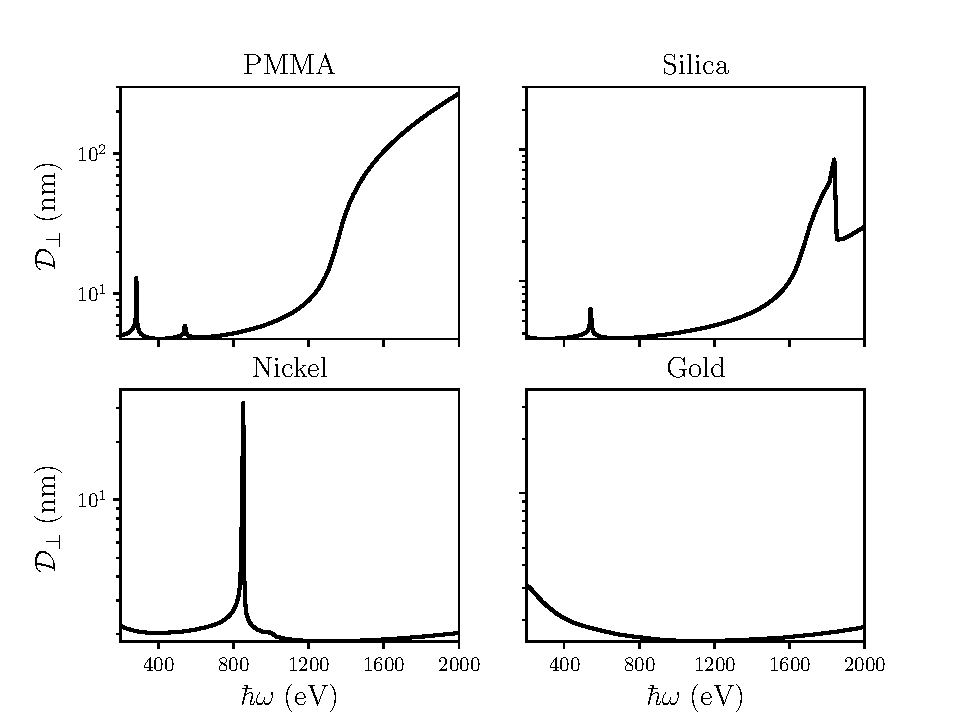
\includegraphics[scale=0.95]{Appendix-C/Figures/X-ray_atten.pdf}
 \caption[TER penetration depth for PMMA, silica, nickel and gold]{TER penetration depth, $\mathcal{D}_{\perp}$, at $\zeta = 1^{\circ}$ for PMMA (\ce{C5H8O2})$_n$, silica (\ce{SiO2}), nickel (\ce{Ni}) and gold (\ce{Au}) \cite{CXRO_database}}\label{fig:X-ray_atten}
 \end{figure} 
This is demonstrated in \cref{fig:X-ray_atten}, where the exact expression for $\mathcal{D}_{\perp}$ using \cref{eq:penetration_depth} with $\zeta = 1^{\circ}$ is plotted across the soft x-ray spectrum for the materials from \cref{fig:X-ray_index,fig:X-ray_lengths,fig:critical_angle,fig:X-ray_refl}. 
It is seen in these plots that $\mathcal{D}_{\perp}$ sharply increases at absorption edges and over other spectral regions where $\zeta \gtrapprox \zeta_c (\omega)$, which is the case for PMMA and silica toward the blue end of the soft x-ray spectrum. 

A mirror flat designed for soft x-rays under TER in practice can be a layer of an appropriate material \numrange{4}{5} $\mathcal{D}_{\perp}$ thick coated on a substrate such as silicon or fused silica. 
Over such a depth, \SIrange{98}{99}{\percent}  of the incident wave intensity is attenuated and as a result, reflections that occur at the interface of the coating and the substrate can be neglected. 
This principle also holds for x-ray reflection gratings, where, as alluded to in \cref{sec:grating_tech_dev}, only a relatively thin layer of a reflective material need be coated on a grating surface relief. 
The penetration depth data from \cref{fig:X-ray_atten} combined with the reflectivity data from \cref{fig:X-ray_refl} indicate that a gold coating provides an efficient, broadband response for grazing-incidence soft x-rays with a relatively thin deposited layer (typically \SIrange{10}{15}{\nm}). 
This is beneficial for x-ray reflection gratings with groove spacings of a few hundred \si{\nm} in terms of diffraction efficiency, both for the overall reflectivity and for maintaining the sawtooth groove shape that affects how efficiency is distributed among propagating orders [\emph{cf.\@} \cref{ch:diff_eff,ap:grating_basics}]. 
Additionally, nickel has similar properties for $\hbar \omega \lessapprox \SI{800}{\electronvolt}$ and may be appropriate in situations where the prominent L-shell absorption edge can be avoided. 

In principle, a thin, reflective overcoat for an x-ray reflection grating can be produced through a variety of chemical vapor or physical vapor deposition techniques \cite{Franssila10}. 
While chemical vapor deposition (especially \emph{atomic layer deposition} \cite{George10}) is advantageous for producing conformal coatings on corrugated surfaces, these processes are very time consuming and therefore become impractical in terms of throughput for spectrometers that require many grating replicas. 
Physical vapor deposition techniques such as \emph{plasma sputtering} or \emph{electron-beam vapor deposition} \cite{Singh05} instead are commonly used for this application with the level of coating conformity depending on the geometry inside the processing chamber. 
The nature of the surface to be coated, however, must be taken into account to ensure that a quality film is produced. 
That is, for a grating mold etched in silicon with native oxide or patterned in resist that contains oxygen, the overcoat material must also be oxidizing to promote wetting and adhesion \cite{Trolier-McKinstry17}. 
While nickel satisfies this condition, gold does not oxidize and therefore a thin film of an oxidizing metal such as chromium or titanium must be first deposited to provide a wetted, metallic surface for a gold layer to adhere to. 
Moreover, the wettability of a reflective overcoat material also contributes to the level of surface roughness on a mirror or similarly, the blazed groove facets of a reflection grating. 

\subsection{Surface Roughness}\label{sec:rough_surface}
%%%%%%%%%%%%%%%%%%%%%%%%%%%%%%%%%%%%%%%%%--------------------------------------------------
Any realistic surface features some level of roughness that, depending on the incident wave vector and the surface profile, serves to reduce specular reflectivity relative to what is predicted by the Fresnel equations [\emph{cf.\@} \cref{sec:reflectivity_polarization}]. 
In principle, a rough surface can be described with a pseudo-random surface profile, $y = Y(x,z)$, where $x$, $y$ and $z$ are the coordinates defined in \cref{fig:2Dmirror_angles} with the average value $\langle Y(x,z) \rangle = 0$ corresponding to a perfectly smooth surface in the plane defined by $y = 0$. 
While the exact analytical form of the function $Y(x,z)$ is unknown in practice, its statistical properties can be used to describe approximately the effect that a rough surface has on incident radiation. 
First, this function fluctuates in value to a level characterized by the variance of $Y(x,z)$:
\begin{equation}\label{eq:surface_variance}
 \sigma^2 \equiv \langle Y^2(x,z) \rangle - \underbrace{\langle Y(x,z) \rangle^2}_0 ,
 \end{equation} 
where $\sigma$ is the \emph{root mean square (RMS) roughness} that describes the typical spread in surface feature heights \cite{Beckmann63,Ogilvy87,Als-Nielsen11,Sentenac2009}.   
Additionally, information on the spread of lateral sizes on the surface is contained within the \emph{autocorrelation function} associated with $Y(x,z)$ \cite{Beckmann63,Hogrefe87,Ogilvy87,Sentenac2009}: 
\begin{equation}\label{eq:auto_correlation}
 C (\mathbold{\tau}) = \frac{\langle Y(\mathbold{\tau}) Y(\mathbf{0}) \rangle}{\sigma^2} ,
 \end{equation}
where $\mathbold{\tau} \equiv \tau_x  \mathbold{\hat{x}} + \tau_z  \mathbold{\hat{z}}$ is a position vector confined to the $y = 0$ plane that represents the directional distance between an arbitrary $(x,z)$ point and an origin $(0,0) \equiv \mathbf{0}$. 

Taking the Fourier transform of \cref{eq:auto_correlation} gives a \emph{power spectral density (PSD) function}, which describes the distribution of spatial frequency components making up the rough surface \cite{Beckmann63,Wen15,Ogilvy87}:
\begin{subequations}
\begin{equation}\label{eq:PSD_general}
 PSD \left( \mathbold{K} \right) = \int_{-\infty}^{\infty} C (\mathbold{\tau}) \, \mathrm{e}^{i \mathbold{K} \cdot \mathbold{\tau}} \dd[2]{\mathbold{\tau}} ,
 \end{equation}
where $\mathbold{K} \equiv K_x  \mathbold{\hat{x}} + K_z  \mathbold{\hat{z}}$ is a spatial analog to $\mathbold{\tau}$. 
The exponential term in the case of an isotropic surface becomes $\mathbold{K} \cdot \mathbold{\tau} = K \tau \cos (\phi)$ with $\tau \equiv |\mathbold{\tau}|$, $K \equiv |\mathbold{K}|$ and $\tan (\phi) \equiv \tau_z / \tau_x$ so that \cref{eq:PSD_general} becomes 
\begin{equation}\label{eq:PSD_isotropic}
 PSD \left( K \right) = \int_{0}^{2 \pi} \int_{0}^{\infty} C (\tau) \, \mathrm{e}^{i K \tau \cos (\phi)} \tau \dd{\tau} \dd{\phi} = 2 \pi \int_{0}^{\infty} C (\tau) \, J_0 \left( K \tau \right) \tau \dd{\tau} ,
 \end{equation}
\end{subequations}
where $J_0 \left(K \tau \right)$ is the $0^{\text{th}}$-order \emph{Bessel function of the first kind}\footnote{Here, \emph{Bessel's first integral} is used with $n=0$: 
\begin{equation*}
 J_n (w) = \frac{1}{2 \pi i^n} \int_0^{2 \pi} \mathrm{e}^{i w \cos (\phi)} \mathrm{e}^{i n \phi} \dd{\phi} .
 \end{equation*}} 
and under this assumption of isotropy, $C (\mathbold{\tau}) = C (\tau)$. 
Moreover, this autocorrelation function is often taken to be a normal distribution: 
\begin{equation}\label{eq:auto_correlation_normal}
 C (\tau) = \mathrm{e}^{- \tau^2 / \ell_{\text{corr}}^2} ,
 \end{equation}
where $\ell_{\text{corr}}$ is the \emph{correlation length}, which is defined by the value of $\tau$ that corresponds to $C (\tau)$ reaching $1/\mathrm{e} \approx \SI{37}{\percent}$ of its maximum value \cite{Beckmann63,Sentenac2009,Ogilvy87,Hogrefe87}. 
Physically, $\ell_{\text{corr}}$ represents a typical size scale of a rough surface feature: $\ell_{\text{corr}} \to 0$ represents very small features that approach white noise while very large $\ell_{\text{corr}}$ indicates the presence of low-frequency surface distortion \cite{Beckmann63,Wen15,Sentenac2009}.

The effect that surface roughness has on incident radiation depends strongly on the typical lateral size scale of surface features, which is characterized by $\ell_{\text{corr}}$. 
If $\sigma$ is small enough however, a surface can be treated as being smooth such that the Fresnel equations for specular reflection given [\emph{cf.\@} \cref{eq:s_reflectivity,eq:p_reflectivity}] are valid. 
While pure specular reflection occurs when the phase of an incident plane wave varies linearly and continuously across a perfectly smooth surface \cite{Jackson75,Born80,Attwood17}, surface roughness with relatively large $\ell_{\text{corr}}$ introduces local phase variations from the differing path lengths that rays take to reflect from the random surface features associated with the roughness \cite{Beckmann63,Ogilvy87}. 
For rays striking two points on a surface that differ in depth by $y = \sigma$ [\emph{cf.\@} \cref{fig:smooth_criterion}], the path-length difference for a specularly reflected wavefront is $\Delta s = 2 \sigma \sin \left( \zeta \right)$, where $\zeta$ is the incidence angle measured relative to the tangent plane of the surface. 
\begin{figure}
 \centering
 \includegraphics{Appendix-C/Figures/scattering2.mps}
 \caption{2D representation of rays incident on a rough surface}\label{fig:smooth_criterion}
 \end{figure} 
The phase shift associated with $\Delta s$ is \cite{Beckmann63,Hogrefe87} 
\begin{subequations}
\begin{equation}\label{eq:roughness_phase}
 \Delta \Phi = k_0 \Delta s = \frac{4 \pi \sigma}{\lambda} \sin \left( \zeta \right) ,
 \end{equation}
which provides a measure of how in-phase specularly reflected light is. 

The level of smoothness for a surface can be quantified by comparing $\Delta \Phi$ to some fixed value, $\Delta \Phi_0$, so that \cref{eq:roughness_phase} can be rearranged to give a requirement on $\sigma$: 
\begin{equation}\label{eq:roughness_inequality_general}
 \sigma < \frac{\Delta \Phi_0 \lambda}{4 \pi \sin \left( \zeta \right)} .
 \end{equation}
\end{subequations}
While the choice of $\Delta \Phi_0$ is somewhat arbitrary, commonly quoted values are $\Delta \Phi_0 = \pi /2$ (the \emph{Rayleigh criterion}) and $\Delta \Phi_0 = \pi /8$ (the \emph{Fraunhofer criterion}) \cite{Beckmann63}. 
Regardless of the exact definition for $\Delta \Phi_0$, the basic principle behind \cref{eq:roughness_inequality_general} can be understood qualitatively by considering the everyday example of the glare that the Sun produces as it reflects from pavement. 
That is, when the Sun is overhead, $\sin \left( \zeta \right) \approx 1$ so that $\sigma < \Delta \Phi_0 \lambda / 4 \pi$ may not be fulfilled for $\SI{700}{\nm} \gtrapprox \lambda \gtrapprox \SI{400}{\nm}$ with typical pavement RMS roughness values. 
On the other hand, pavement can appear smooth to sunlight with sufficiently small $\zeta$ when the Sun is low in the sky, which results in a glare that comes from specular reflection. 
For soft x-rays with $\SI{5}{\nm} \gtrapprox \lambda \gtrapprox \SI{0.5}{\nm}$, these conditions have much tighter constraints but at grazing-incidence angles in the regime of TER, high-quality surfaces with sufficiently small $\sigma$ can be regarded as being smooth to incident radiation. 
Using the Fraunhofer criterion and taking $\zeta = 1^{\circ}$ as a typical graze angle, \cref{eq:roughness_inequality_general} becomes $\sigma \lessapprox 1.8 \lambda$, which suggests that nanoscale values of $\sigma$ are needed to realize a smooth surface for grazing-incidence soft x-rays. 

\subsubsection{Debye-Waller Regime}\label{sec:DW_factor}
%%%%%%%%%%%%%%%%%%%%%%%%%%%%%%%%%%%%%%%%%--------------------------------------------------
The scenario described in the preceding paragraph relies on the assumption of $\ell_{\text{corr}}$ being large enough such that the electromagnetic fields at the boundary of the surface can be defined locally in a precise way. 
In the context of soft x-rays and other radiation with $\nu (\omega) = 1 - \delta_{\nu} (\omega) \lessapprox 1$, this condition is considered fulfilled when $\ell_{\text{corr}} \gg \ell_{\text{ext}}$, with $\ell_{\text{ext}} \equiv \lambda / 2 \pi \delta_{\nu} (\omega)$ being the extinction length \cref{eq:extinction_length} \cite[\emph{cf.\@} \cref{eq:extinction_length}]{deBergevin09,Gibaud2009}. 
Determining how the incident electromagnetic fields respond to a rough surface in principle requires solving the Helmholtz equations given by \cref{eq:Helmholtz_above_mirror,eq:Helmholtz_below_mirror} using boundary conditions that are a generalization of \cref{eq:general_boundary_1,eq:general_boundary_2,eq:general_boundary_3,eq:general_boundary_4} for a perfectly smooth surface: 
\begin{subequations}
\begin{align}
 \mathbold{\hat{n}} \times \left[ \mathbold{E} \left( x, Y(x,z), z \right) + \mathbold{E''} \left( x, Y(x,z), z \right) \right] &= \mathbold{\hat{n}} \times \mathbold{E'} \left( x, Y(x,z), z \right) \label{eq:rough_boundary_1} \\
 \mathbold{\hat{n}} \times \left[\mathbold{H} \left( x, Y(x,z), z \right)  + \mathbold{H''} \left( x, Y(x,z), z \right) \right] &= \mathbold{\hat{n}} \times \mathbold{H'} \left( x, Y(x,z), z \right)  \label{eq:rough_boundary_2} \\
 \mathbold{\hat{n}} \cdot \left[ \mathbold{E} \left( x, Y(x,z), z \right) + \mathbold{E''} \left( x, Y(x,z), z \right) \right] &= \tilde{\nu}^2 (\omega) \, \mathbold{\hat{n}} \cdot \mathbold{E'} \left( x, Y(x,z), z \right) \label{eq:rough_boundary_3} \\
 \mathbold{\hat{n}} \cdot \left[ \mathbold{H} \left( x, Y(x,z), z \right) + \mathbold{H''} \left( x, Y(x,z), z \right) \right] &= \mathbold{\hat{n}} \cdot \mathbold{H'} \left( x, Y(x,z), z \right) \label{eq:rough_boundary_4} , 
 \end{align}
\end{subequations}
where $Y(x,z)$ describes the rough surface profile and $\mathbold{\hat{n}} \equiv \mathbold{\hat{n}} (x,z)$ is a unit vector normal to the tangent plane of a roughness feature located at a point $(x,z)$. 
While this is in general a very complicated problem, the \emph{tangent-plane approximation} can be invoked for $\ell_{\text{corr}} \gg \ell_{\text{ext}}$ such that $Y(x,z)$ varies slow enough to make the assumption $\mathbold{\hat{n}} (x,z) \approx \mathbold{\hat{y}}$. 

In the tangent-plane approximation, \cref{eq:rough_boundary_1,eq:rough_boundary_2,eq:rough_boundary_3,eq:rough_boundary_4} for s-polarization\footnote{Because the expressions for Fresnel reflectivity in orthogonal polarizations, $\mathcal{R}_s$ and $\mathcal{R}_p$, are virtually equal at grazing incidence [\emph{cf.\@} \cref{fig:X-ray_refl}], only s-polarization need be considered here.} yield the following two relations after taking into account Snell's law that mandates $k_x = k_x'' = \tilde{k_x}' = k_0 \cos (\zeta)$ and $k_z = k_z'' = \tilde{k_z}' \equiv 0$: 
\begin{subequations}
\begin{align}
 \mathcal{A}_s \mathrm{e}^{i k_y Y(x,z)} + \mathcal{A}_s'' \mathrm{e}^{-i k_y Y(x,z)} &= \mathcal{A}_s' \mathrm{e}^{i \tilde{k_y}' Y(x,z)} \label{eq:tangent_plane1} \\
 \mathcal{A}_s k_y \mathrm{e}^{i k_y Y(x,z)} - \mathcal{A}_s'' k_y \mathrm{e}^{-i k_y Y(x,z)} &= \mathcal{A}_s' \tilde{k_y}' \mathrm{e}^{i \tilde{k_y}' Y(x,z)} \label{eq:tangent_plane2}
 \end{align}
\end{subequations}
with $\mathcal{A}_s$, $\mathcal{A}_s''$ and $\mathcal{A}_s'$ being the amplitudes of the incident, reflected and refracted wavefronts, respectively, while $k_y = -k_0 \sin (\zeta)$ and $\tilde{k_y}' = -k_0 \sqrt{\tilde{\nu}^2 (\omega) - \cos^2 (\zeta)}$. 
These two equations can be solved for the reflected amplitude: 
\begin{equation}
 \mathcal{A}_s'' = \mathcal{A}_s \mathrm{e}^{2 i k_y Y(x,z)} \left( \frac{k_y - \tilde{k_y}'}{\tilde{k_y}' + k_y} \right)
 \end{equation}
and using this relation, a reduced reflectivity can be defined as 
\begin{subequations}
\begin{equation}\label{eq:DW_refl_s}
 \mathcal{R}_{DW} \equiv \norm{\frac{\langle \mathcal{A}_s'' \rangle}{\mathcal{A}_s}}^2 = \norm{\langle \mathrm{e}^{2 i k_y Y(x,z)} \rangle}^2 \underbrace{\norm{\left( \frac{k_y - \tilde{k_y}'}{\tilde{k_y}' + k_y} \right) }^2 }_{\mathcal{R}_s} , %= \mathrm{e}^{-2 k_y^2 \sigma^2} ,
 \end{equation}
where, assuming that the randomness of the surface profile, $Y(x,z)$, is described by a normal distribution\footnote{For a random variable $X$ that is described by a Gaussian distribution, the \emph{Baker-Hausdorff theorem} states that $\langle \mathrm{e}^{i X} \rangle = \mathrm{e}^{-\frac{1}{2} \langle X^2 \rangle}$ \cite{Als-Nielsen11}. Moreover, $\sigma^2 \equiv \langle Y^2 (x,z) \rangle$ from \cref{eq:surface_variance}.} and using the definition of $\sigma^2$ in \cref{eq:surface_variance},
\begin{equation}\label{eq:DW_factor}
 \langle \mathrm{e}^{2 i k_y Y(x,z)} \rangle = \mathrm{e}^{-2 k_y^2 \langle Y^2(x,z) \rangle} = \mathrm{e}^{-2 k_y^2 \sigma^2}
 \end{equation}
\end{subequations}
is known as the \emph{Debye-Waller factor} \cite{Gibaud2009}. 
With the under-braced term in \cref{eq:DW_refl_s} recognized as $\mathcal{R}_F$ for s-polarization, \cref{eq:DW_factor} is equivalent to the fraction of radiation lost to surface roughness for large $\ell_{\text{corr}}$, $\mathcal{R}_{DW} / \mathcal{R}_F = \mathrm{e}^{-4 k_y^2 \sigma^2}$. 

\subsubsection{Intermediate Regime}\label{sec:intermediate_rough}
%%%%%%%%%%%%%%%%%%%%%%%%%%%%%%%%%%%%%%%%%--------------------------------------------------
For a surface assumed to be dominated by features with a large $\ell_{\text{corr}}$ such that the Debye-Waller factor is valid, the reduction in specular reflectivity is attributed to diffuse scatter in vacuum with the total integrated scatter being equal to $1 - \mathrm{e}^{-4 k_y^2 \sigma^2}$ \cite{Wen15}. 
While this expression breaks down as $\ell_{\text{corr}}$ decreases\footnote{This occurs when the tangent-plane approximation is no longer valid such that the boundary conditions given by \cref{eq:rough_boundary_1,eq:rough_boundary_2,eq:rough_boundary_3,eq:rough_boundary_4} must be applied for an arbitrary normal vector $\mathbold{\hat{n}} (x,z)$.} and does not describe how the intensity of scattered light is distributed, this behavior can be understood in part by considering a rough surface to be a superposition of sinusoidal components with various periods and orientations described by the vector $\mathbold{K}$ introduced for the the PSD function [\emph{cf.\@} \cref{eq:PSD_general}]. 
Defining $\abs{\mathbold{K}} \equiv K \equiv 2 \pi / \Lambda$, a single mode of a rough surface in principle acts as a sinusoidal reflection grating with a groove spacing equal to $\Lambda$, which is an effective \emph{surface wavelength} \cite{Cash87,Sentenac2009,Aschenbach85}. 
Approximate scattering behavior then can be gleaned by considering how an electromagnetic wave interacts with such a structure for 
\begin{enumerate}[noitemsep]
  \item the exact \emph{in-plane} case, where the plane defined by the incident wave vector, $\mathbold{k}$, and $\mathbold{K}$ is perpendicular to the surface defined by $y=0$, and 
  \item the totally \emph{off-plane} case, where $\mathbold{k}$ is perpendicular to $\mathbold{K}$.
 \end{enumerate}

The locations of diffracted orders for a grating for an oblique incidence angle are described by the \emph{generalized grating equation} [\emph{cf.\@} \cref{eq:off-plane_incidence_orders,eq:off-plane_orders}]: 
\begin{equation} \label{eq:grating_rough}
 \sin \left( \alpha \right) + \sin \left( \beta \right) = \frac{n \lambda}{\Lambda \sin \left( \gamma \right)} ,
 \end{equation}
where $\alpha$ is the polar incidence angle, $\beta$ is the polar diffracted angle of the $n^{\text{th}}$ order and $\gamma$ is the cone-opening angle of the diffraction pattern [\emph{cf.\@} \cref{fig:conical_reflection_edit,fig:conical_reflection}]. 
For the in-plane scenario [\emph{cf.\@} \cref{fig:in_plane_scatter}], all diffracted orders are confined to this same plane with $\sin (\gamma) = 1$ so that the incidence angle measured relative to the surface is $\zeta = \pi / 2 - \alpha$. 
\begin{figure}
 \centering
 \includegraphics[scale=1.0]{Appendix-C/Figures/diffraction_arc10.mps}
 \caption{In-plane scatter from a single mode of surface roughness}\label{fig:in_plane_scatter}
 \end{figure}
The diffracted angle moreover is taken to be $\beta = \Delta \beta - \alpha$, where $\Delta \beta$ is the angular deviation from specular for the scattered ray, so that 
\cref{eq:grating_rough} becomes 
\begin{subequations}
\begin{equation}
 \cos \left( \zeta \right) - \cos \left( \Delta \beta + \zeta \right) = \frac{n \lambda}{\Lambda} .
 \end{equation}
Using a trigonometric identity\footnote{$\cos \left( \Delta \beta + \zeta \right) = \cos \left( \Delta \beta \right) \cos \left( \zeta \right) - \sin \left( \Delta \beta \right) \sin \left( \zeta \right)$} and taking $n=1$ for first-order diffraction\footnote{According to the scalar treatment of diffraction described in \cref{sec:sinusoid_principle}, diffracted orders with $n = \pm 1$ are expected to dominate over those with larger $\abs{n}$.} gives 
\begin{equation}
 \frac{\lambda}{\Lambda} = \underbrace{\cos \left( \zeta \right)}_{\approx 1} \left[ 1 - \underbrace{\cos \left( \Delta \beta \right)}_{\approx 1} \right] + \underbrace{\sin \left( \zeta \right)}_{\approx \zeta} \underbrace{\sin \left( \Delta \beta \right)}_{\approx \Delta \beta} , %\approx \zeta \Delta \beta ,  
 \end{equation}
where, using the under-braced small-angle approximations for a grazing-incidence angle $\zeta \ll 1$, the scattered angle is 
\begin{equation}\label{eq:in-plane_scatter_angle}
 \Delta \beta \approx \frac{\lambda}{\zeta \Lambda} .
 \end{equation}
\end{subequations}

The scenario for the off-plane case [\emph{cf.\@} \cref{fig:off_plane_scatter}] corresponds to $\alpha = 0$, $\beta =  \Delta \beta $ and $\gamma = \zeta$ with all diffracted orders confined to the surface of a cone so that \cref{eq:grating_rough} becomes 
\begin{subequations}
\begin{equation} 
 \underbrace{\sin \left( \zeta \right)}_{\approx \zeta} \underbrace{\sin \left( \Delta \beta \right)}_{\approx \Delta \beta} = \frac{n \lambda}{\Lambda} , 
 \end{equation}
where the under-braced approximations hold for small angles. 
\begin{figure}
 \centering
 \includegraphics[scale=1.0]{Appendix-C/Figures/diffraction_arc11.mps}
 \caption{Off-plane scatter from a single mode of surface roughness}\label{fig:off_plane_scatter}
 \end{figure}
In this case, however, the off-plane scattered angle is $\varphi''$ that is labeled in \cref{fig:off_plane_scatter} and defined by the following relation:
\begin{equation}
 \sin \left( \varphi'' \right) = \tan \left( \zeta \right) \tan \left( \Delta \beta \right) ,
 \end{equation}
which can be approximated as $\varphi'' \approx \zeta \Delta \beta$. 
Taking $n=1$ for first-order diffraction, this diffracted angle can be expressed as 
\begin{equation}\label{eq:off-plane_scatter_angle}
 \varphi'' \approx \frac{\lambda}{\Lambda} .
 \end{equation}
\end{subequations}
Comparing \cref{eq:in-plane_scatter_angle,eq:off-plane_scatter_angle} shows that the angular spread of in-plane scattering is $\zeta^{-1}$ times larger than that of off-plane scattering assuming $\zeta \ll 1$ for grazing-incidence soft x-rays \cite{Aschenbach85}.
This suggests that diffuse scattering produced by a rough surface is most detrimental for an x-ray reflection grating in the plane defined by the incident wave vector and the direction normal to the active blazed groove facets \cite{Cash87}. 
However, determining the intensity of scattered radiation requires the use of more rigorous techniques such as the \emph{distorted-wave Born approximation} \cite{Vineyard82,Sinha88,Vinogradov85,Daillant2009}. 

\subsubsection{Nevot-Croce Regime}\label{sec:NC_factor}
%%%%%%%%%%%%%%%%%%%%%%%%%%%%%%%%%%%%%%%%%--------------------------------------------------
Beyond diffuse scattering vacuum, specular reflectivity can also be reduced due to absorption, as radiation scatters into the depth of the reflective material that makes up a rough surface. 
This predominately occurs when $\ell_{\text{corr}}$ is so small that typical values for $\Lambda$ do not produce diffraction by \cref{eq:grating_rough} for the generalized grating equation \cite{deBoer95}. 
In the case of a surface with $\ell_{\text{corr}} \ll \ell_{\text{ext}}$, there is no precise phase relationship at the boundary $Y (x,z)$ and instead, the boundary conditions defined by \cref{eq:rough_boundary_1,eq:rough_boundary_2,eq:rough_boundary_3,eq:rough_boundary_4} are met only on average so that \cref{eq:tangent_plane1,eq:tangent_plane2} for the tangent-plane approximation are again valid, but only for \emph{effective amplitudes} \cite{Gibaud2009}. 
To show this, multiplying \cref{eq:tangent_plane1} by $k_y$ gives 
\begin{subequations}
\begin{align}
 \mathcal{A}_s k_y \mathrm{e}^{i k_y Y(x,z)} + \mathcal{A}_s'' k_y \mathrm{e}^{-i k_y Y(x,z)} &= \mathcal{A}_s' k_y \mathrm{e}^{i \tilde{k_y}' Y(x,z)} \label{eq:tangent_plane1_eff} \\
 \mathcal{A}_s k_y \mathrm{e}^{i k_y Y(x,z)} - \mathcal{A}_s'' k_y \mathrm{e}^{-i k_y Y(x,z)} &= \mathcal{A}_s' \tilde{k_y}' \mathrm{e}^{i \tilde{k_y}' Y(x,z)} \label{eq:tangent_plane2_eff} 
 \end{align}
\end{subequations}
while adding the two relations and subtracting \cref{eq:tangent_plane2_eff} from \cref{eq:tangent_plane2_eff} yields 
\begin{subequations}
\begin{align}
 2 \mathcal{A}_s k_y \mathrm{e}^{i k_y Y(x,z)} &= \mathcal{A}_s' \left( k_y + \tilde{k_y}' \right) \mathrm{e}^{i \tilde{k_y}' Y(x,z)}  \label{eq:tangent_plane1_eff_comb} \\
 2 \mathcal{A}_s'' k_y \mathrm{e}^{-i k_y Y(x,z)} &= \mathcal{A}_s' \left( k_y - \tilde{k_y}' \right) \mathrm{e}^{i \tilde{k_y}' Y(x,z)}  \label{eq:tangent_plane2_eff_comb} .
 \end{align}
\end{subequations}

The effective amplitudes on the boundary correspond to average values with \cref{eq:tangent_plane1_eff_comb,eq:tangent_plane2_eff_comb} rewritten as
\begin{subequations}
\begin{align}
 \langle \mathcal{A}_s \rangle &= \frac{1}{2 k_y} \langle \mathcal{A}_s' \rangle \left( k_y + \tilde{k_y}' \right) \langle \mathrm{e}^{i \left( \tilde{k_y}' - k_y \right) Y(x,z)} \rangle \label{eq:tangent_plane1_eff_comb_alt} \\
 \langle \mathcal{A}_s'' \rangle  &= \frac{1}{2 k_y} \langle \mathcal{A}_s' \rangle \left( k_y - \tilde{k_y}' \right) \langle \mathrm{e}^{i \left( \tilde{k_y}' + k_y \right) Y(x,z)} \rangle \label{eq:tangent_plane2_eff_comb_alt} 
 \end{align}
\end{subequations}
with the reduced reflectivity given by\footnote{Similar to the derivation of the Debye-Waller factor, it is again assumed that $Y(x,z)$ is a random variable described by Gaussian distribution so that the following relation holds: $\langle \mathrm{e}^{i X} \rangle = \mathrm{e}^{-\frac{1}{2} \langle X^2 \rangle}$ \cite{Als-Nielsen11}.} 
\begin{subequations}
\begin{equation}
 \mathcal{R}_{NC} \equiv \norm{\frac{\langle \mathcal{A}_s'' \rangle}{\langle \mathcal{A}_s \rangle}}^2 = \norm{\frac{\langle \mathrm{e}^{i \left( \tilde{k_y}' + k_y \right) Y(x,z)} \rangle}{\langle \mathrm{e}^{i \left( \tilde{k_y}' - k_y \right) Y(x,z)} \rangle}}^2 \underbrace{\norm{\left( \frac{k_y - \tilde{k_y}'}{\tilde{k_y}' + k_y} \right)}^2}_{\mathcal{R}_s} , \label{eq:NC_refl_s}
 \end{equation}
where
\begin{equation}
 \frac{\langle \mathrm{e}^{i \left( \tilde{k_y}' + k_y \right) Y(x,z)} \rangle}{\langle \mathrm{e}^{i \left( \tilde{k_y}' - k_y \right) Y(x,z)} \rangle} = \frac{\mathrm{e}^{- \frac{1}{2} \left( \tilde{k_y}' + k_y \right)^2 \langle Y^2 (x,z) \rangle}}{\mathrm{e}^{- \frac{1}{2} \left( \tilde{k_y}' - k_y \right)^2 \langle Y^2 (x,z) \rangle}} = \mathrm{e}^{- 2 k_y \tilde{k_y}' \sigma^2}
 \end{equation}
is a complex quantity known as the \emph{Nevot-Croce factor} \cite{Gibaud2009,deBoer95,Wen15,Nevot80}. 
With $\mathcal{R}_s$ for Fresnel reflectivity recognized in \cref{eq:NC_refl_s}, the fraction of specularly reflected radiation lost due to absorption can be written as 
\begin{equation}\label{eq:NC_refl_ratio}
 \frac{\mathcal{R}_{NC}}{\mathcal{R}_F} = \norm{\mathrm{e}^{- 2 k_y \tilde{k_y}' \sigma^2}}^2 = \mathrm{e}^{-2 k_y \left( \tilde{k_y}' + \tilde{k_y}'^* \right) \sigma^2} = \mathrm{e}^{-4 k_0^2 \sin \left( \zeta \right) \Re \left[ \sqrt{\tilde{\nu}^2 (\omega) - \cos^2 \left( \zeta \right) } \right] \sigma^2}
 \end{equation}
for a thick slab, where again, $\mathcal{R}_F \approx \mathcal{R}_s \approx \mathcal{R}_p$ for grazing-incidence soft x-rays of any polarization [\emph{cf.\@} \cref{sec:reflectivity_polarization}]. 
\end{subequations}
Treating reduced specular reflectivity using Nevot-Croce factors is considered a decent approximation if surface features with relatively large lateral sizes can be ignored while atomic-scale features with small $\sigma$ dominate surface roughness. 
In any case, the effect that a rough surface has on the specular reflectivity of a mirror flat is analogous to the losses in diffracted orders that result from surface roughness on the blazed groove facets of an x-ray reflection grating. % and therefore, this phenomenon must be kept under control to achieve high diffraction efficiency. 

\section{Summary}\label{sec:appC_summary}
%%%%%%%%%%%%%%%%%%%%%%%%%%%%%%%%%%%%%%%%%--------------------------------------------------
Due to the fact that their photon energy range, \SI{250}{\electronvolt}~$\lessapprox \mathcal{E}_{\gamma} \lessapprox$~\SI{2}{\kilo\electronvolt}, coincides with the spectrum of K-shell binding energies in low-to-mid $\mathcal{Z}$ atoms while their wavelength range, \SI{5}{\nm}~$\gtrapprox \lambda \gtrapprox$~\SI{0.5}{\nm}, approaches the atomic scale, soft x-rays are easily absorbed by $\mathcal{Z} \geq 6$ materials and additionally, appreciable reflectivity from a surface can only be achieved at grazing-incidence angles, $\zeta$, that are smaller than the critical angle for total external reflection (TER), $\zeta_c (\omega)$. 
Although materials with moderate $\mathcal{Z}$ (\emph{e.g.}, nickel) may provide high reflectivity over a limited bandpass, those with high $\mathcal{Z}$ (\emph{e.g.}, gold) tend to offer broadband reflectivity at soft x-ray wavelengths. 
These phenomena can be gleaned from the complex index of refraction for a given material, $\tilde{\nu} (\omega) = \nu (\omega) + i \xi (\omega)$, 
where $\nu (\omega) \equiv 1 - \delta_{\nu} (\omega) \lessapprox 1$ leads to $\zeta_c (\omega) \approx \sqrt{2 \delta_{\nu} (\omega)}$ with $\delta_{\nu} (\omega) \ll 1$ while $\xi (\omega) \neq 0$ gives rise to reflectivity losses and in turn, a nonzero penetration depth, $\mathcal{D}_{\perp}$, that informs thickness requirements for deposited, reflective films used in the soft x-ray. 
A film \numrange{4}{5} $\mathcal{D}_{\perp}$ thick (typically $\sim \SI{15}{\nm}$) effectively functions as a thick slab, and with Fresnel reflectivity being virtually polarization-insensitive in the regime of TER, the quantity need only be calculated for a single polarization. 
Finally, effects of nanoscale surface roughness in the limit of small and large correlation length, $\ell_{\text{corr}}$, can be modeled using Nevot-Croce and Debye-Waller factors, respectively, while the intermediate region requires more advanced treatment. 